\documentclass[12pt,a4paper,openany]{book}
%------------------------------------------------------------------------------------------------------------------------------------------------------------------------------------------------------------------------------
% PACKAGES
%--------------------------------------------------------------------------------------------------------------------------------------------------------------------------------------------------------------------------------

% Selección de idioma
\usepackage[spanish]{babel}

% algo
\usepackage[utf8]{inputenc}

% Par acomodar la foto del editorial
\usepackage{wrapfig}

% Paquetes útiles
\usepackage[table]{xcolor}
\usepackage{amssymb}
\usepackage{amsmath}
%\usepackage{mathbbol}
\usepackage{bbm}
\usepackage{amsthm}
\usepackage{pdfpages}
\usepackage{graphicx,color,psfrag}
\usepackage{epstopdf}
\usepackage{pdflscape}
\usepackage{tabularx}
\usepackage{longtable}
\usepackage{breakurl}
\usepackage{enumitem}
\usepackage[normalem]{ulem}
\usepackage{blindtext}
\usepackage{mathtools,breqn}


\usepackage{fancyhdr}
\usepackage{graphicx}

\usepackage{fnpct}

\usepackage{subcaption}

\usepackage{newpxtext}
\usepackage{lscape}

% La mejor fuente de la letra: https://www3.gobiernodecanarias.org/medusa/ecoblog/lortrodm/files/2015/03/tarea-formatos-word.pdf
% caption fonts
%\usepackage[font={large,bf}]{caption} 
\usepackage[T1]{fontenc}
\usepackage{verdana}


\usepackage{setspace}
\usepackage{longtable}
\usepackage{threeparttable}  
\usepackage{tabulary}
\usepackage{booktabs}
\usepackage{float}
\usepackage{caption}
\usepackage{subcaption}
\usepackage{rotating}
\usepackage[titletoc,title]{appendix}

\usepackage{array,multirow}

\usepackage[round]{natbib}
\bibpunct{(}{)}{;}{a}{,}{;}
\setcounter{MaxMatrixCols}{10}

\topmargin=-1.8cm \textheight=23.8cm \oddsidemargin=-0.3cm
\evensidemargin=-0.5cm \textwidth=17.1cm

\newtheorem{theorem}{Theorem}
\newtheorem{corollary}[theorem]{Corollary}
\newtheorem{proposition}{Proposition}
\newtheorem{assumption}{Assumption}
\newtheorem{assumption2}{Assumption A}

\newtheorem{lemma}{Lemma}

\usepackage{tikz}
\usetikzlibrary{positioning}
\tikzset{>=stealth}
\usepackage{amsmath}
\usepackage{verbatim}
\usetikzlibrary{arrows,shapes}

% Definir colores
\definecolor{mycolor1}{RGB}{221, 165, 230}
\definecolor{mycolor2}{RGB}{54, 56, 120}	
\definecolor{mycolor3}{RGB}{205, 24, 24}
\definecolor{mycolor4}{RGB}{164, 93, 93}
\definecolor{mycolor5}{RGB}{243, 149, 13}
\definecolor{mycolor6}{RGB}{3, 83, 151}
\definecolor{mycolor7}{RGB}{52, 103, 81}
\usepackage[colorlinks=true,linkcolor=myblue, allcolors=mycolor2]{hyperref}
\usepackage{soul}

% Tablas
\usepackage{tabularx}
\usepackage{multirow}
\usepackage{multicol} 
\usepackage{booktabs}%\usepackage{booktabs, calc} %This is the package to use to have nice-looking tables. More documentation on the tables in LateX: https://www.tug.org/pracjourn/2007-1/mori/mori.pdf
\usepackage{threeparttable} 

\usepackage{lmodern}
\usepackage{booktabs}
\usepackage{pgfplots}

\graphicspath{{../figuras/}}

\begin{document}
	
	%---------------------------------------------------------------------------
	% TITLE PAGE
	%---------------------------------------------------------------------------
	\doublespacing
	
	\title{Boletín COVID-19}
	\author{Autores}
	
	\date{}

	%\maketitle
	
	
	%\thispagestyle{empty}\baselineskip1.385\baselineskip \newpage{}
	
	\pagestyle{plain}\pagenumbering{arabic}
	
	%insertar el cover
	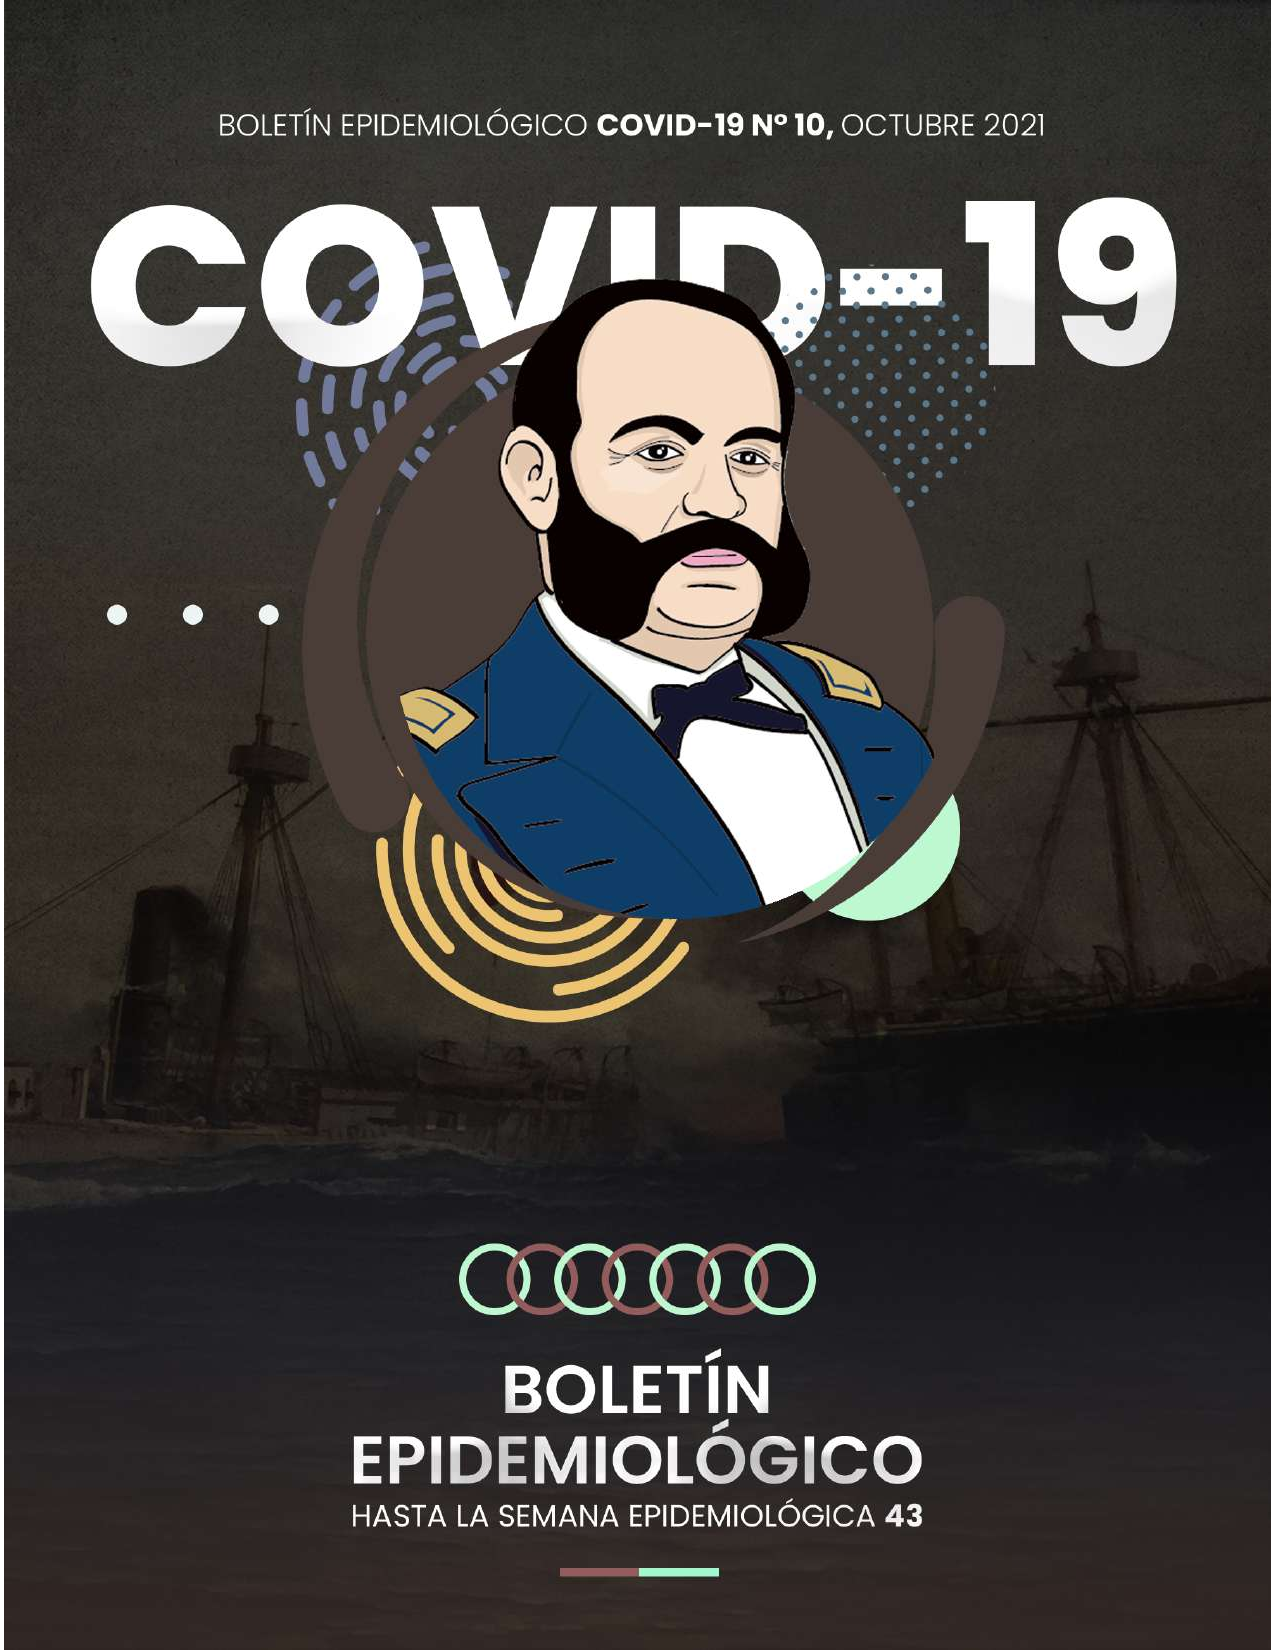
\includepdf[pages={1}]{../editorial/portada.pdf}
	\clearpage
	
	\pagestyle{plain}\pagenumbering{arabic}
	
	\clearpage
	
	
	\begin{center}
	
		{\large Gerencia Regional de Salud}
		
		\textbf{MSP. Javier Ramírez Escóbar}
		
		Gerente Regional \vspace{1.0cm}
		
		Dirección Ejecutiva de Inteligencia Sanitaria
		
		\textbf{MSP. Darío Francisco Navarro Mendoza}
		
		Director
		
		\vspace{1.5cm}
\noindent
\begin{minipage}[t]{.45\textwidth}
	\centering
	Dirección de Epidemiología e Investigación  \\
	\textbf{MSC. Fátima R. Concha Velasco}\\
	Directora \vspace{1.0cm}\\
	% Por orden alfabético del apellido
	\textit{Equipo de Epidemiología e Investigación }\vspace{.5cm}\\
	Econ. Karen Yorka Aguilar Zuñiga \\
	Lic. Nadia Isabel Cáceres Pillco \\
	TAP. Edgar Waldo Capcha Salcedo \\
	M.S.P. Pablo Fidel Grajeda Ancca \\
	M.C. Alex Jaramillo Corrales \\ 
	M.C. Katia Luque Quispe \\
	M.C. Ana Gabriela Eulalia Moncada Arias \\
	M.C. Jesus Kevin Perez Castilla \\
	Lic. Enf. Ruth Nelly Oscco Abarca \\
	Ing. Joel Wilfredo Sumerente Ayerbe \\
	Lic. Enf. Guinetta Margarita Yabar Herrera \vspace{1.5cm}\\	
\end{minipage}
\hfill
\noindent
\begin{minipage}[t]{.45\textwidth}
	\centering
	Dirección de Estadística, Informática y Telecomunicaciones\\
	\textbf{Ing. Abel Rimasca Chacón} \\
	Director \vspace{1.0cm} \\
	% Por orden alfabético del apellido
	\textit{Equipo de Estadística, Informática y Telecomunicaciones} \vspace{.5cm} \\
	Ing. Iván Atayupanqui Rondón \\
	Ing. Miguel Ángel Campana Alarcón \\
	Ing. Uriel Lacuta Farfán \\
	Ing. Jorge Fernando Lovatón Ramos \\
	Ing. Danny Robert Moscoso Sánchez \\
	Lic. Ray Milton Valderrama Álverez \vspace{1.5cm}\\
\end{minipage}
Secretaria: Sra. Ruth Baca Mendoza
	\end{center}
\let\cleardoublepage\clearpage
	\tableofcontents
\begin{center}
Visite nuestro Dashboard interactivo sobre COVID-19 haciendo clic \href{https://geresacusco.shinyapps.io/DASHBOARD\_COVID-19\_CUSCO/}{AQUÍ}
\end{center}
	
	%\mainmatter
	%---------------------------------------------------------------------------
	% CAPÍTULO: EDITORIAL
	%---------------------------------------------------------------------------

	\pagebreak
	
	\section*{Editorial}	\addcontentsline{toc}{chapter}{Editorial}
			\begin{wrapfigure}{l}{8.5cm}
		\label{wrap-fig:1}
		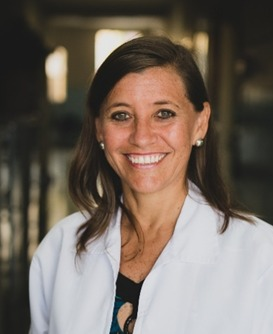
\includegraphics[width=8.5cm]{../editorial/editorial_ochoa}
		\caption*{
			\centering
			Theresa J. Ochoa, MD, PhD.			
			\textit{ Directora del Instituto de Medicina Tropical Alexander von Humboldt-
				Universidad Peruana Cayetano Heredia}
			
		}
	\end{wrapfigure}
	\noindent \textbf{Recomendaciones para el inicio escolar en tiempos  de COVID-19}

En nuestro país esta semana los niños han iniciado el retorno a las escuelas. En las siguientes semanas se espera que todas las instituciones educativas a nivel nacional inicien sus actividades presenciales. Este es un gran hito en el Perú, dado que la mayoría de estudiantes han estado  más de 600 días sin clases presenciales, representando un gran impacto en su aprendizaje, desarrollo y salud mental.  Vemos con mucha alegría y optimismo este retorno escolar.

Actualmente estamos en la etapa final de la tercera ola del COVID-19.  La peculiaridad de esta ola es la predominancia de la variante Omicron, que se caracteriza por una alta contagiosidad e infectividad, pero que en general produce una infección más leve. Esta infección se caracteriza por síntomas respiratorios altos, menor frecuencia de compromiso pulmonar, y menor riesgo de hospitalización, ingreso a cuidados intensivos y requerimiento de ventilación mecánica.  

Si bien  la infección de COVID-19 es menos frecuente en niños y adolescentes, (representa alrededor del 5 $\%$ del total de infectados), y es menos letal (<0.5$\%$), en lo que va de la pandemia, se han infectado en el Perú alrededor de 80,000 niños menores de 5 años y han fallecido, lamentablemente, alrededor  de 800 niños en este grupo de edad. Los más afectados son los niños con co-morbilidades. Por lo tanto, debemos aún seguir cuidando a nuestros niños y debemos  enfatizar algunas recomendaciones para un retorno seguro  a la escuela. 

\textbf{Lo primero es recordar que lo más importante es estar al día con la vacunación contra el COVID-19}, tanto en los adultos (profesores, personal administrativo, de seguridad, de limpieza) como en los adolescentes y niños que están en la edad de vacunarse.  \textbf{Es importante que los adultos tengan sus tres dosis} (dos dosis más el refuerzo), dado que la protección contra el Omicron es mayor con la tercera dosis, sobre todo para evitar infección severa, hospitalización y muerte. En Enero del 2022 iniciamos en el Perú la vacunación a niños entre 5 y 11 años; sin embargo, la cobertura de vacunación en este grupo de edad es aún muy baja. Debemos recordar que la vacunación de los niños ofrece una capa adicional de protección  para evitar que  ellos desarrollen infección severa u hospitalización. Por lo tanto, debemos alentar a los padres a que lleven a vacunar a sus hijos. Recordar que la vacuna es segura, bien tolerada y eficaz para prevenir COVID-19 severo.      

En segundo lugar debemos cumplir con los protocolos establecidos en los centros educativos. Estos protocolos deben adaptarse  a cada realidad escolar. Debemos además recordar que estos deben ir modificándose según como vaya el desarrollo de la pandemia y la nueva evidencia científica que respalda las decisiones en salud pública. Aún no sabemos cómo será el comportamiento del virus y la pandemia en los meses venideros.

Los profesores, alumnos y padres de familia deben \textbf{recordar el ABCD para el retorno seguro}: 


•	\textbf{A de Aseo}. Lavado de manos o uso de alcohol gel, para evitar la transmisión de enfermedades infecciosas en general, no solo COVID-19 sino también otras enfermedades como resfríos, neumonía, diarrea.


•	\textbf{B de Boca}. Usar la mascarilla que cubra boca y nariz, para evitar el contagio del SARS-CoV2. El único momento en que los niños se pueden retirar la mascarilla es para la hora de la  lonchera,  intentando en la medida de lo posible que esto se realice al aire libre o en espacios muy ventilados. 


•\textbf{	C de Casa}. Los niños o profesores que estén enfermos, o que tengan un familiar enfermo o con sospecha de COVID-19, deben quedarse en casa para evitar el contagio. Deben quedarse en casa aún sin que se haya confirmado la infección, pues debemos recordar que el mayor contagio se da en los primeros días de la infección. Pasado 7 días pueden regresar a la escuela. Es mucho más seguro y eficaz implementar  esta medida, para evitar futuros  contagios y brotes en la escuela; sin embargo, esta medida requiere de mucha responsabilidad personal. 


•\textbf{	D de Distanciamiento}.  En la medida de lo posible se debe mantener la distancia de un metro entre niño y niño, propiciando la buena ventilación de las aulas, manteniendo puertas y ventanas abiertas, y tratando de tener la mayor cantidad de actividades al aire libre.  

Es importante recordar que de todas maneras se van a dar contagios de COVID-19 (es inevitable),  lo crítico es minimizar los contagios y evitar los  brotes. Si un niño se contagia de COVID-19 (o si se sospecha) debe avisar al  maestro lo más pronto posible y debe quedarse en casa. Si un niño tiene COVID-19 debe aislarse en casa 7 días. Si un niño ha estado en contacto con alguien con COVID-9, debe hacer cuarentena en casa por 7 días. El manejo en la casa es similar al manejo de un resfrió: paracetamol para la fiebre y el malestar, y buena hidratación. Los síntomas con la variante actual, en la mayoría de los casos duran 3-4 días. Debemos estar atentos a los signos de alarma: fiebre persistente, dificultad respiratoria, disminución en la saturación del oxígeno, compromiso del sensorio (somnolencia, mareos), diarrea, vómitos persistentes y difíciles de manejar en el hogar. En estos casos, se debe acudir inmediatamente a un establecimiento de salud.

En resumen, nos unimos al  júbilo de millones de niños y adolescentes que retornan este mes a la presencialidad, deseado un retorno  seguro,  organizado y progresivo que permita ajustar los protocolos a cada circunstancia y realidad escolar.  
\begin{figure}[htb]
	\centering
	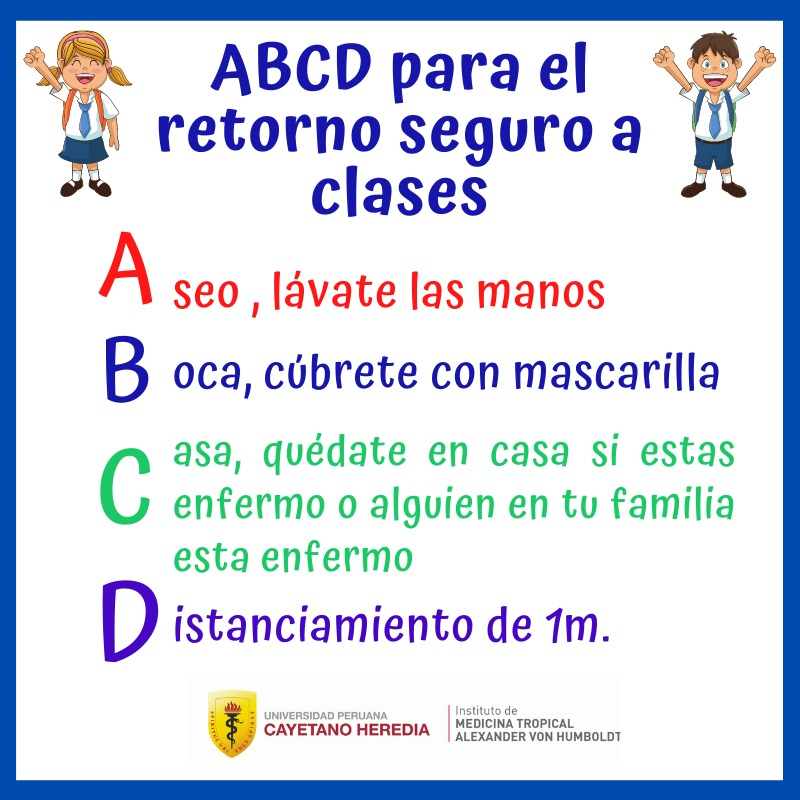
\includegraphics[width=8cm]{../editorial/editorial_abc}
	\caption*{ ABCD para el retorno a clases}
\end{figure}


	
	%---------------------------------------------------------------------------
	% CAPÍTULO: METODOLOGÍA
	%---------------------------------------------------------------------------
			%insertar el cover del capitulo
	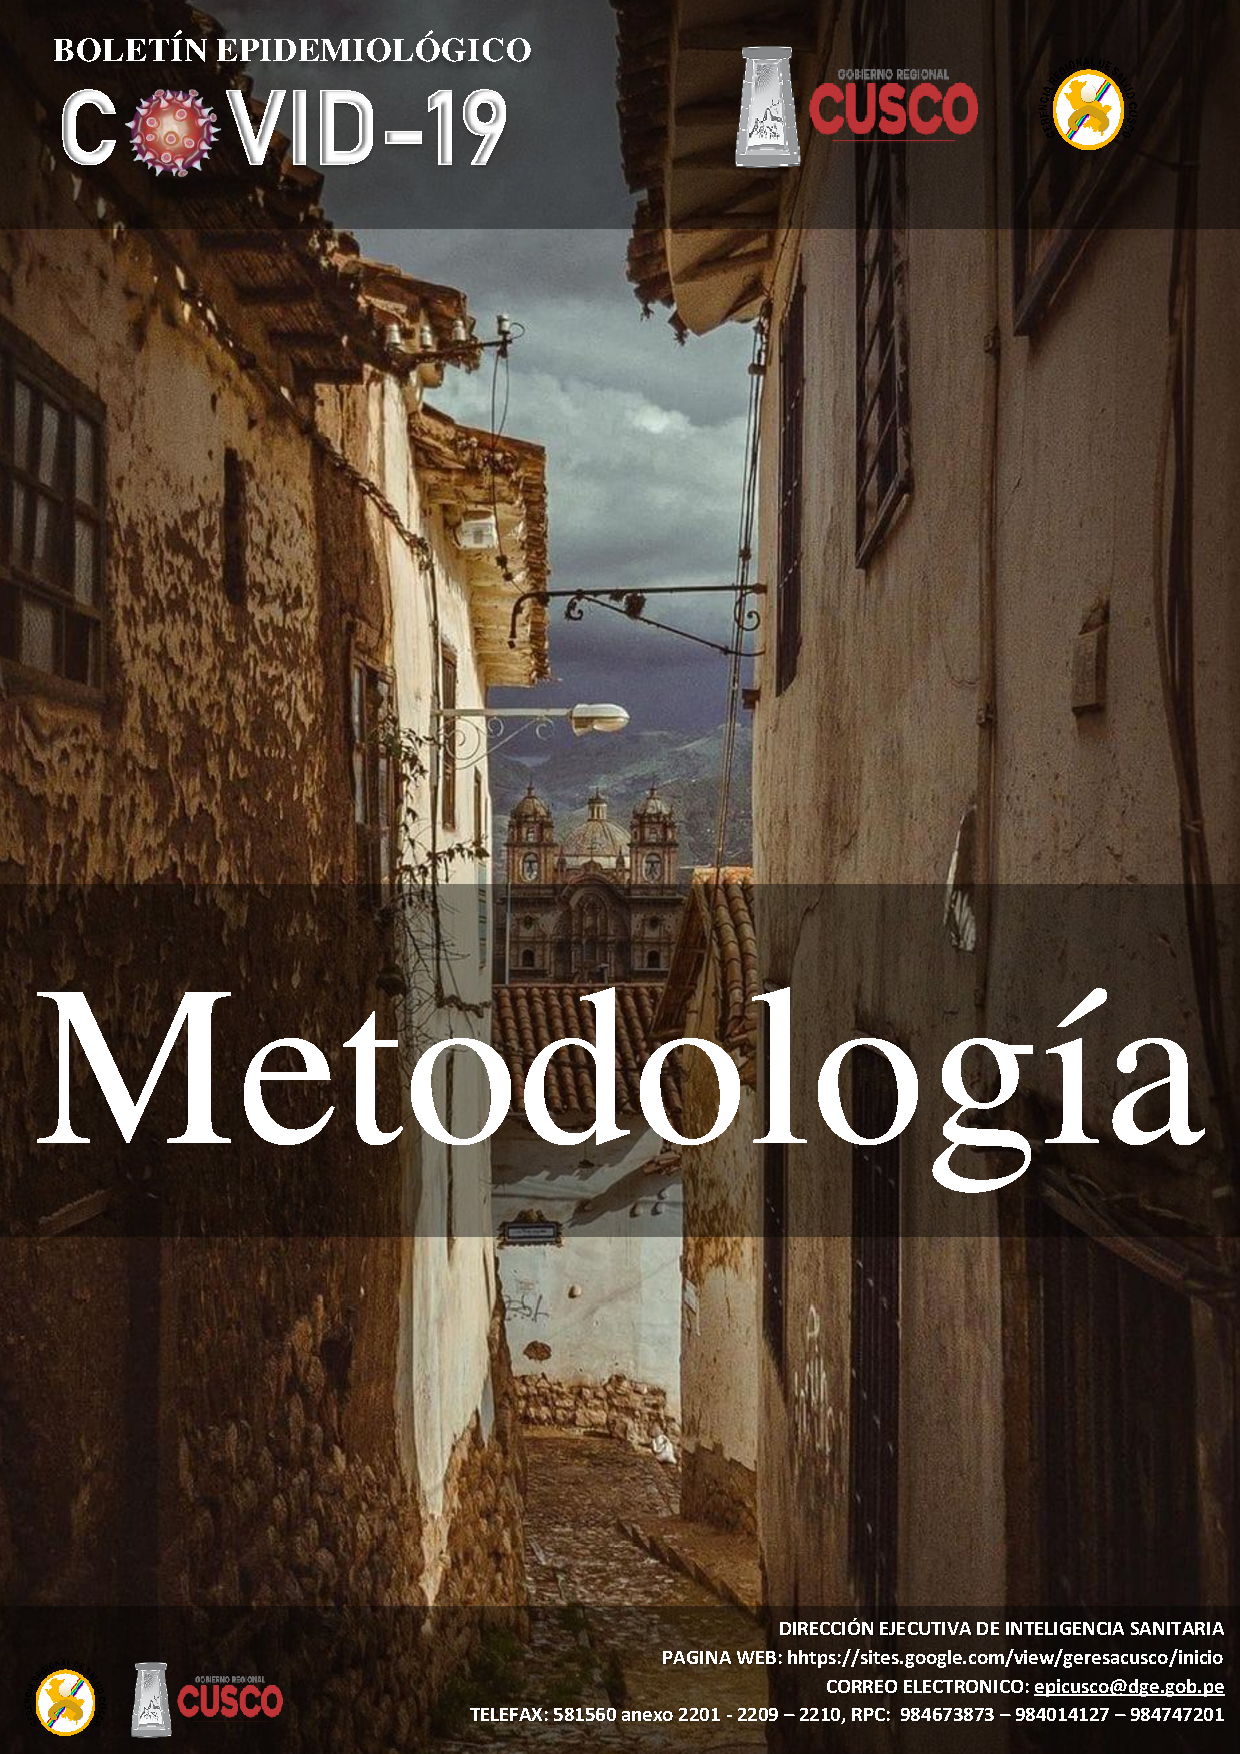
\includepdf[pages={1}]{../editorial/1.pdf}
	\clearpage
	
	\section*{Metodología}	
	\addcontentsline{toc}{chapter}{Metodología}
	\noindent El presente Boletín tiene el objetivo de informar sobre los principales indicadores epidemiológicos y de gestión hospitalaria,  para hacer el seguimiento de la pandemia en nuestra región y tomar mejores decisiones. Este Boletín tiene una metodología de tipo descriptiva. 
	
	La introdución de la variante ómicron en nuestra región ha marcado el inicio de la tercera ola pandémica, es por esto que en esta edición del boletín se considera los datos desde el año 2021 hasta la semana epidemiológica 7 (21 de febrero del 2022), para que el lector pueda hacer las comparaciones e inferencia del comportamiento de la segunda ola y la tercera ola, actualmente en fase de descenso en nuestra región. Asimismo, en la descripción de cada indicador o figura se indicará si el análisis de la información incluye otro periodo. 
	
	Los datos analizados incluyeron: a) características generales: sexo, edad, casos confirmados, fallecidos; b) características clínicas: síntomas reportados, casos confirmados sintomáticos, casos confirmados asintomáticos y comorbilidades; c) indicadores epidemiológicos: sistema de vigilancia epidemiológica, tasa de mortalidad, tasa de positividad de pruebas diagnósticas, casos activos – recuperados, y exceso de muerte por todas las causas, y d) indicadores de gestión hospitalaria: , ocupación de camas UCI y No UCI en la Región. En este boletín se considera como caso positivo de COVID-19, sólo a aquellos que tienen una prueba antigénica o molecular positiva, salvo en ciertas estimaciones, en cuya descripción se detalla si se utilizó otro tipo de examen diagnóstico. 
	
	Las fuentes de información son las bases de datos de NOTI WEB (aplicativo del Sistema de Vigilancia Epidemiológica - COVID-19), SISCOVID (Sistema Integrado para COVID-19), SINADEF (Sistema Informático Nacional de Defunciones), SICOVAC-HIS MINSA(Base de datos de vacunación por COVID-19), Reporte de Disponibilidad de Camas de Hospitalización y datos de la Oficina de Referencias-Contrarreferencias de la Dirección de Emergencias y Desastres de GERESA-Cusco. 
	
	Se usaron frecuencias absolutas y relativas para la descripción de los datos cualitativos. Para la descripción de datos cuantitativos se calcularon tasas (mortalidad, pruebas diagnósticas, incidencia de casos), promedios (ocupación de camas hospitalarias, fallecidos por COVID y fallecidos por todas las causas). Para describir la tendencia se representaron los datos cuantitativos y frecuencias relativas en intervalos de 7 días (semana epidemiológica). En las variables de sistema de vigilancia epidemiológica (1 prueba por 100,000 habitantes) y ocupación de cama (adecuado, menor a $70\%$, moderado, entre $75$ a $90\%$ y limitado, más de $90\%$), siendo todos los puntos de referencia sugeridos por la Organización Mundial de la Salud. Para el análisis de exceso de mortalidad, se usó la metodología descrita por C. Giattino, H. Ritchie, M. Roser, E. Ortiz-Ospina, y J. Hasell en el artículo "Excess mortality during the Coronavirus pandemic (COVID-19)". Published online at OurWorldInData.org.
	
	La descripción de dichas variables se hace de manera regional y provincial. En la presente edición se hace una descripción de la tasa de incidencia, tasa de mortalidad, tasa de positividad por prueba molecular y antigénica, y exceso de defunciones de todas las provincias de nuestra región. El lector interesado en un análisis distrital de los casos y defunciones puede encontrar dicha información en los links correspondientes.
	
	La novedad de esta edición es la inclusión de los datos de la población pediátrica afectada por COVID-19 y un análisis de la supervivencia de los hospitalizados con COVID-19 en la región.
	 
	%---------------------------------------------------------------------------
	% CAPÍTULO: CARACTERÍSTICAS GENERALES
	%---------------------------------------------------------------------------
		%insertar el cover del capitulo
	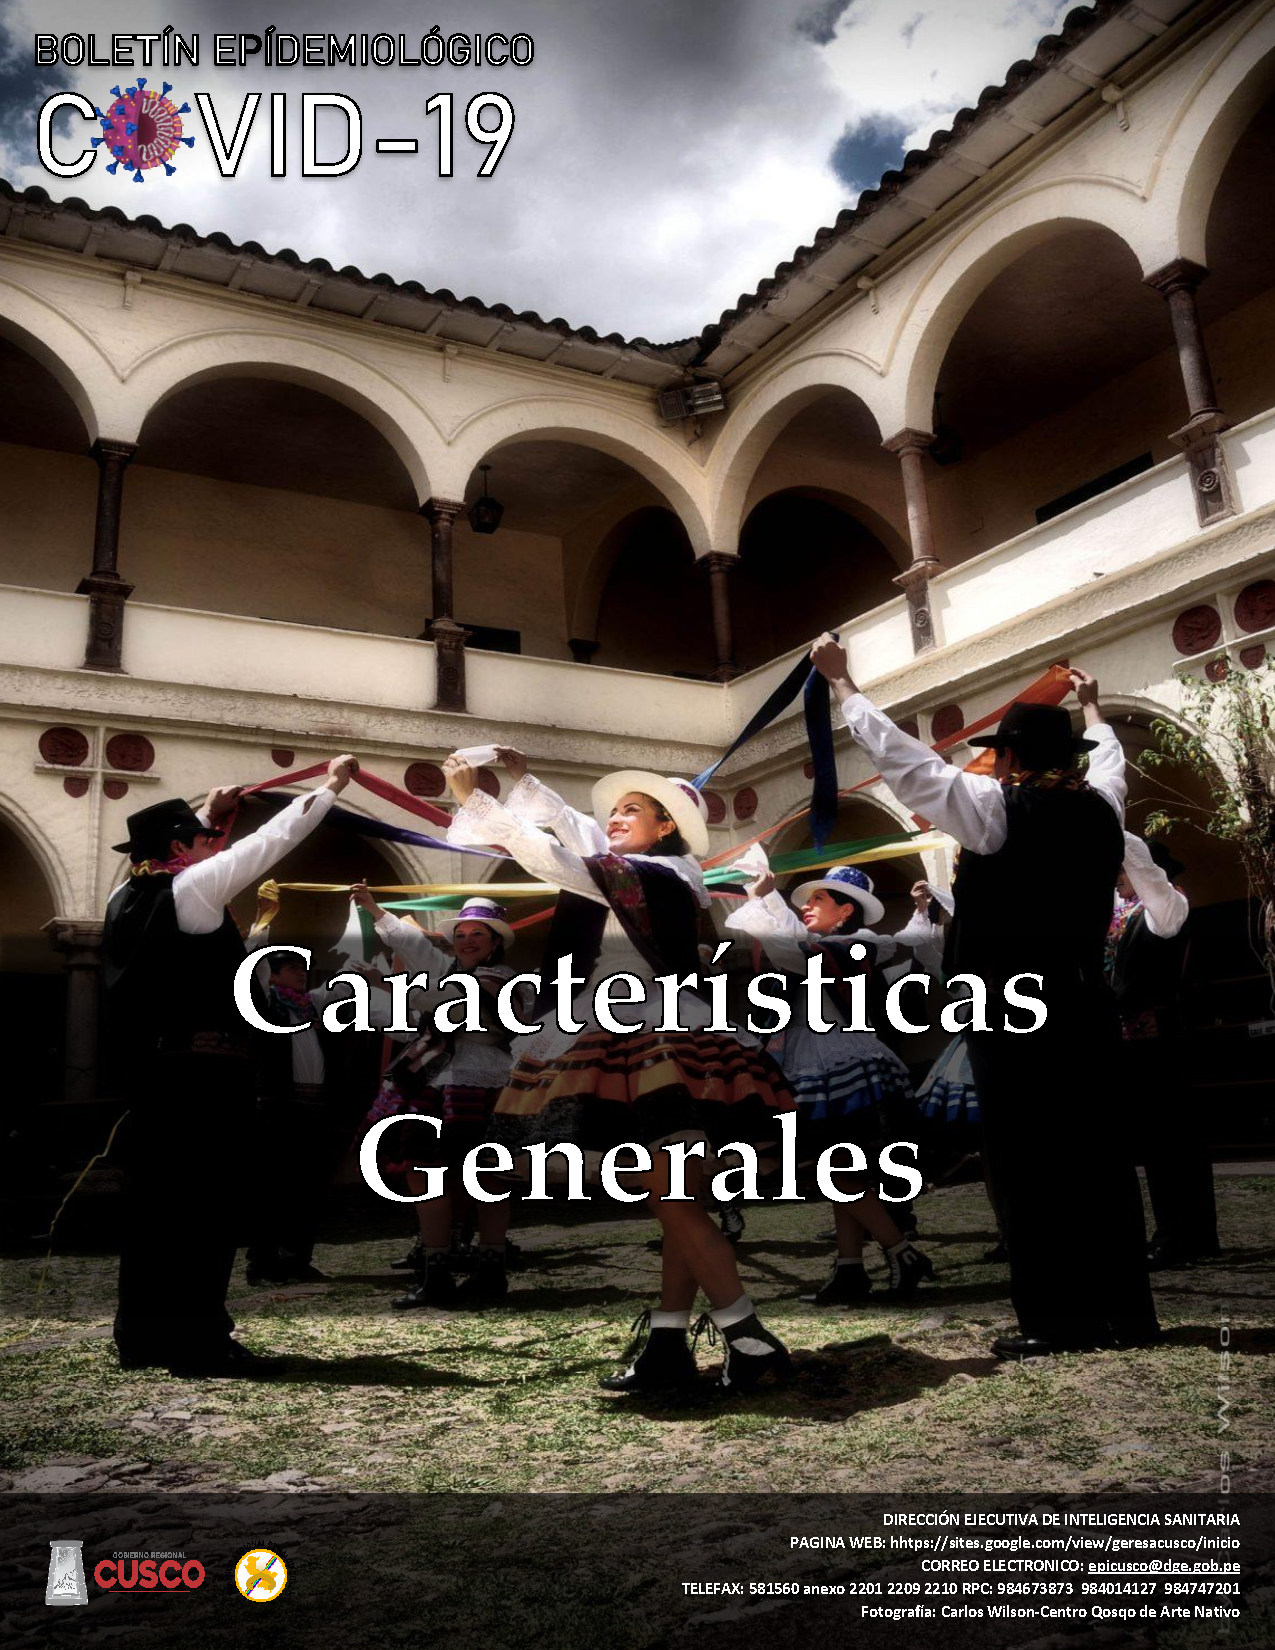
\includepdf[pages={1}]{../editorial/2.pdf}
	\clearpage	
	\section*{Características Generales}
	\addcontentsline{toc}{chapter}{Características Generales}
	
	
	
 	\noindent En la Figura \ref{fig:casos_edad_sexo} se muestra la cantidad de casos confirmados de COVID-19, por prueba antigénica o molecular por grupo etario (en intervalos de 10 años) y sexo. Se observa que la mayor cantidad de casos diagnosticados se concentra en el grupo etario de 30 a 39 años( 11 931  casos acumulados), con mayor afectación del sexo femenino, seguido del grupo etario de 20 a 29 años (11 567 casos acumulados) con el mayor número de casos en e mismo sexo del grupo previo. Es importante recalcar que la cantidad de niños afectados de 0 a 9 años (1 088 casos acumulados) sigue en ascenso y el acumulado es mayor al registrado en los anteriores años.  
 	
 	
\begin{figure}[h]
	\caption{Casos Confirmados de COVID-19 según Grupo de Edad y Sexo en la Región Cusco hasta la SE 07-2022(*).}\label{fig:casos_edad_sexo}
	\begin{center}
		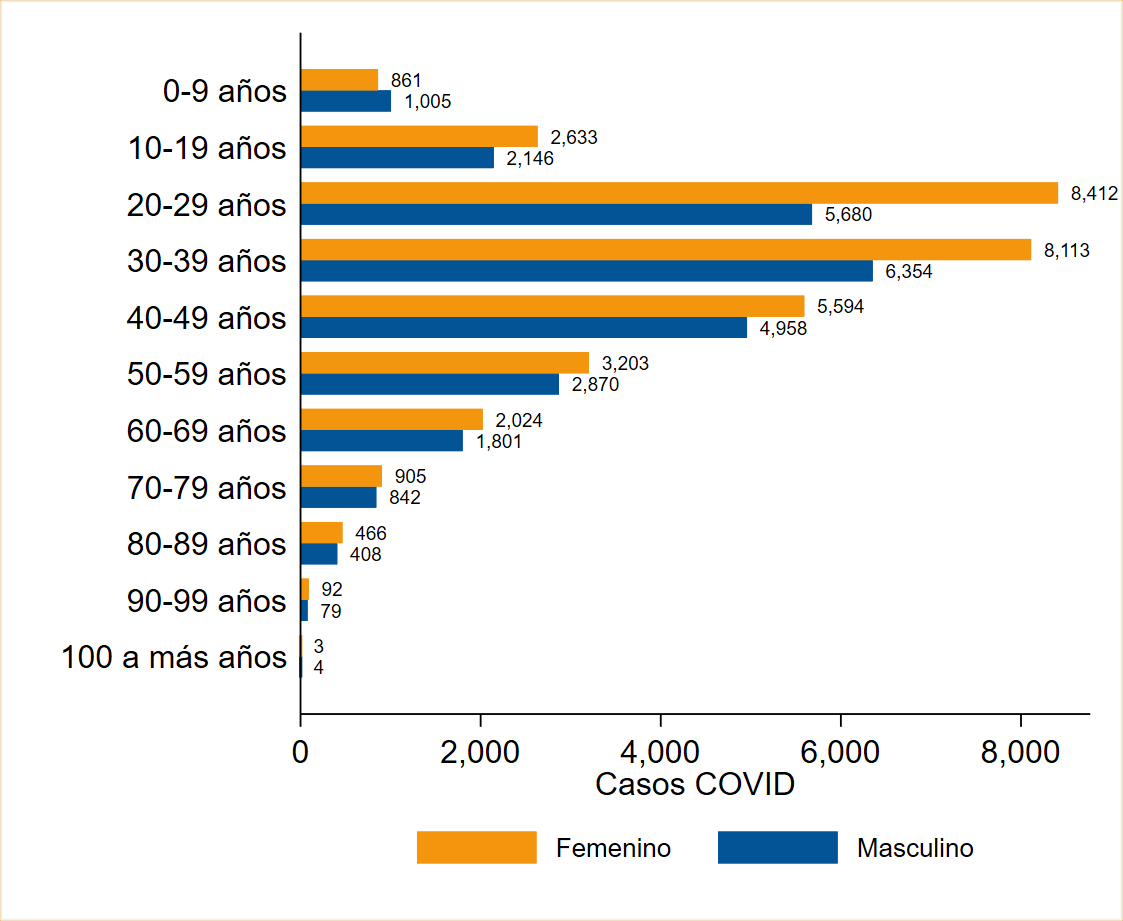
\includegraphics[width=0.75\linewidth]{../figuras/casos_etapavida_2022}
	\end{center}
	{\footnotesize {Fuente de datos: SISCOVID, NOTICOVID.(*)Sólo se incluye información del 2022.}}
\end{figure}
\pagebreak


La Figura \ref{fig:fallecidos_edad_sexo}  muestra el número de muertes reportadas por COVID-19 conforme al grupo etario y sexo hasta el 21 de febrero del 2022, se observa que el mayor número de muertes se registra en el grupo etario de 80 a 89 años (60 muertes acumuladas) con un mayor número de muertes del sexo femenino, seguido del grupo etario de 70 a 79 años (29 muertes acumuladas). En este reporte la cantidad de fallecidos de sexo femenino (88 muertes reportadas) supera a la cantidad de fallecidos de sexo masculino (79 muertes reportadas). 

\begin{figure}[h]
	\caption{Casos fallecidos por COVID-19 según Grupo Etario y Sexo en la Región Cusco hasta la SE 07-2022(*).}\label{fig:fallecidos_edad_sexo}
	\begin{center}
		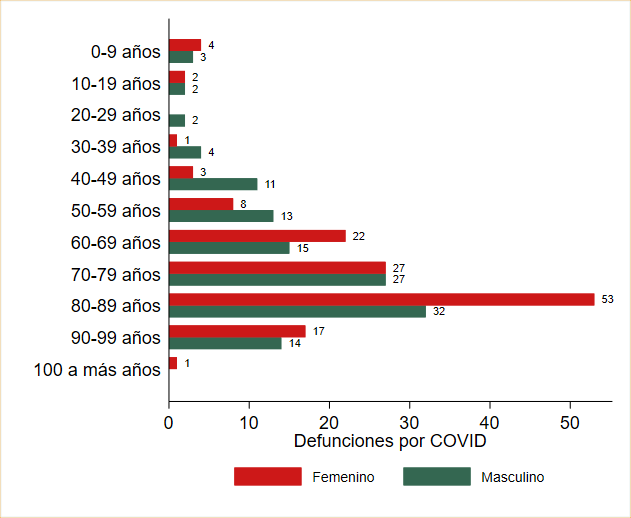
\includegraphics[width=0.75\linewidth]{../figuras/defunciones_etapavida_2022}
	\end{center}
	{\footnotesize {Fuente de datos: SISCOVID, NOTICOVID.(*) Sólo se incluye información del 2022.}}
\end{figure}



\cleardoublepage
%---------------------------------------------------------------------------
% CAPÍTULO: CARACTERÍSTICAS CLÍNICAS
%---------------------------------------------------------------------------
	%insertar el cover del capitulo
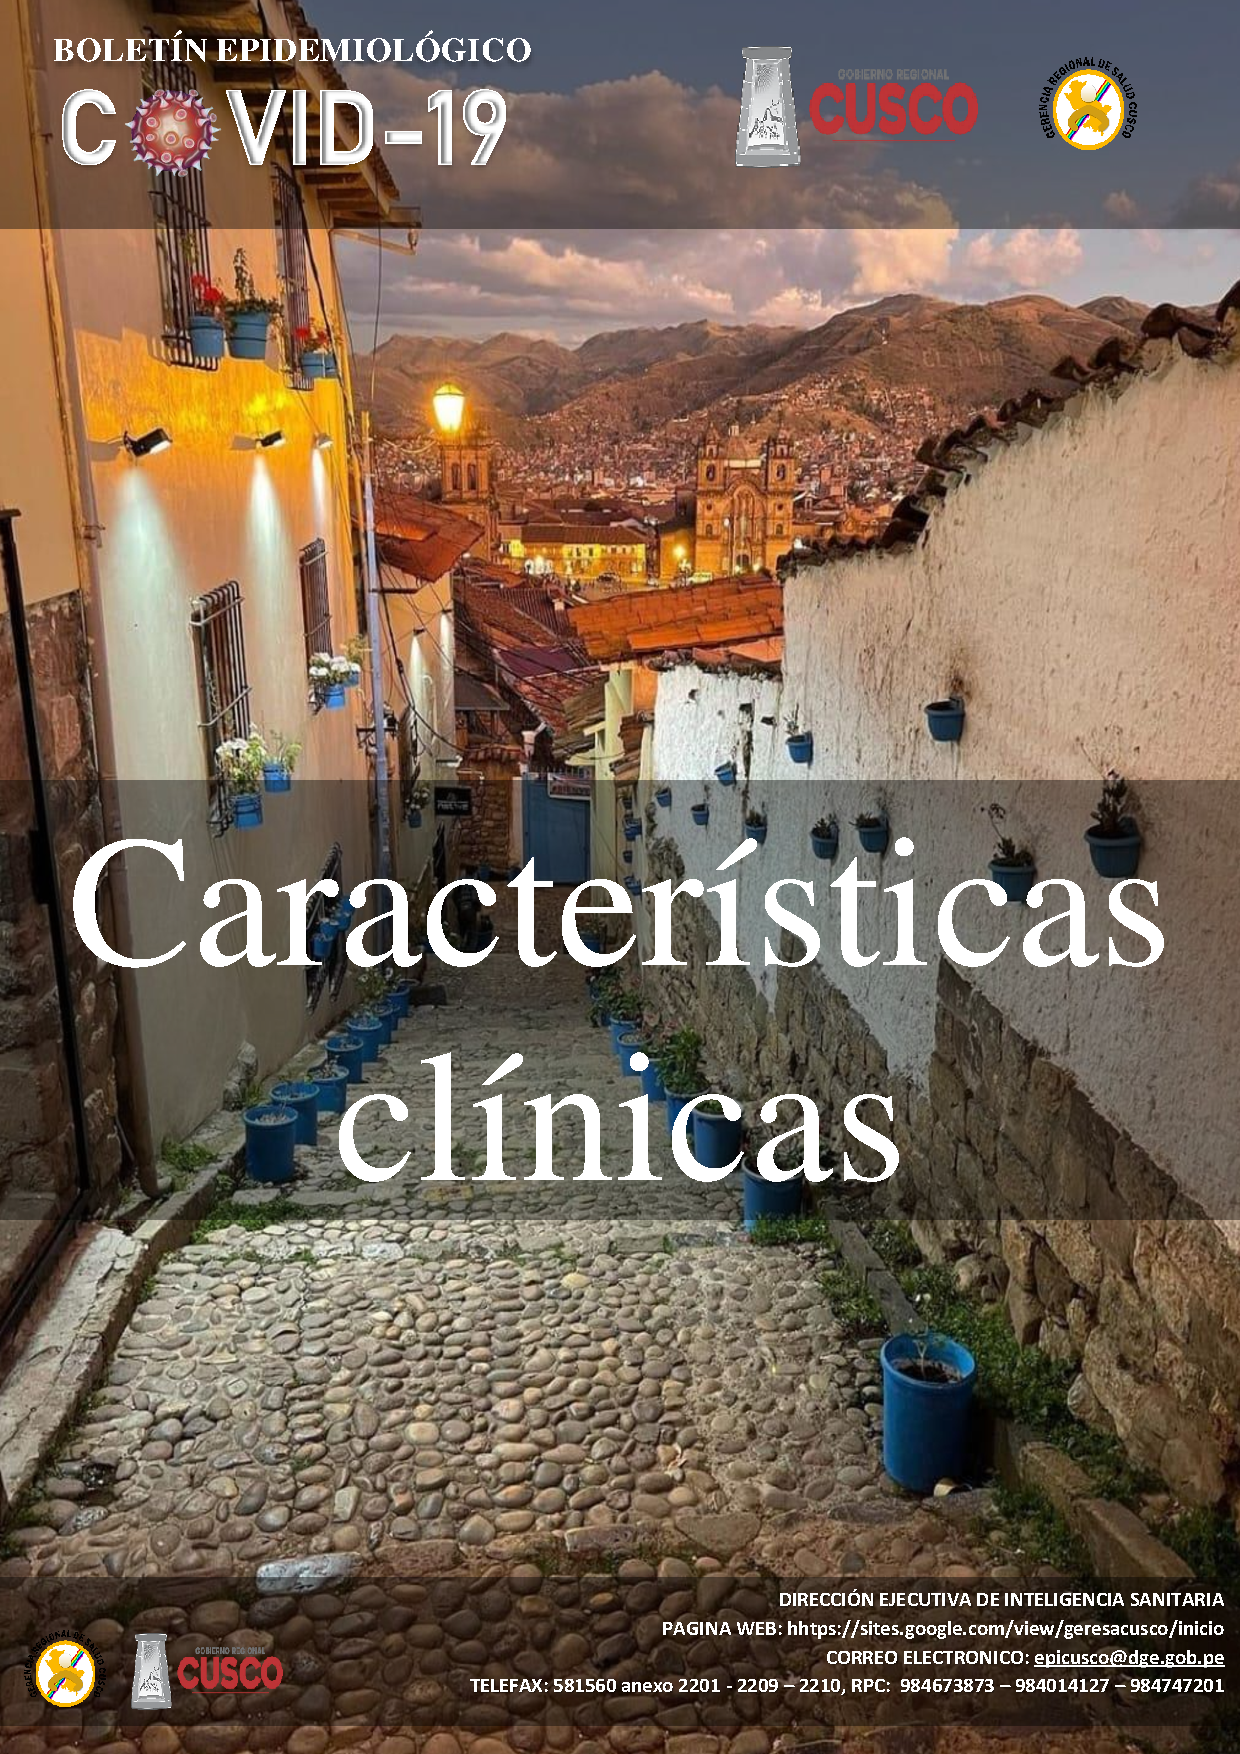
\includepdf[pages={1}]{../editorial/3.pdf}

\clearpage

\section*{Características Clínicas}
\addcontentsline{toc}{chapter}{Características Clínicas}	
\noindent En la Figura \ref{fig:sintomas} se presentan los síntomas más frecuentes autorreportados por los pacientes con diagnóstico de COVID-19, el dolor de garganta (18,8 $\%$) es el síntomas más reportado, seguido de tos (18,0 $\%$) y malestar (13,5$\%$). Dentro de los signos más frecuentes (Figura \ref{fig:signos}), el exudado faríngeo constituye el signo más prevalente (84,9$\%$). 

\begin{figure}[h]
	\caption{Síntomas más frecuentes de los pacientes diagnosticados por COVID-19 en la Región Cusco hasta la SE 07-2022.  }\label{fig:sintomas}
	\begin{center}
		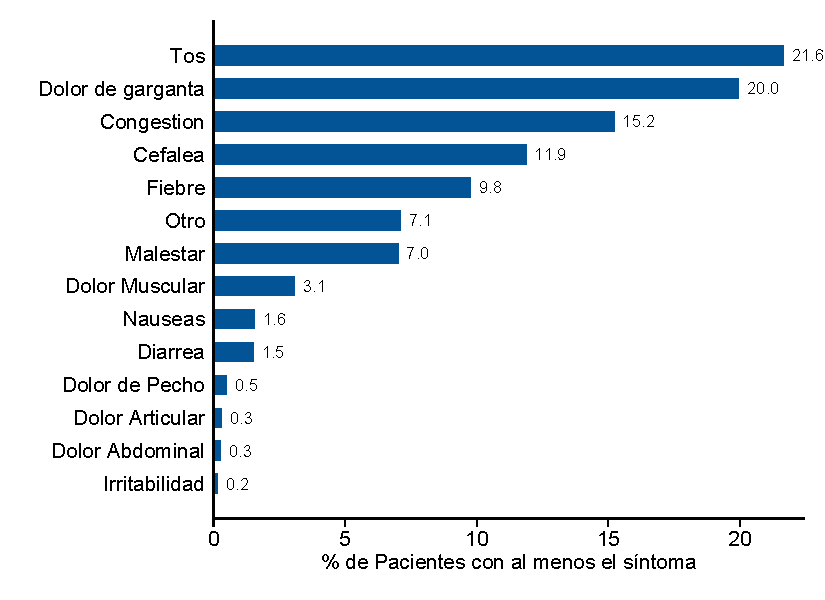
\includegraphics[width=0.85\linewidth]{../figuras/figura_sintoma.pdf}
	\end{center}
	{\footnotesize {Fuente de datos: SISCOVID, NOTICOVID.}}
\end{figure}

\begin{figure}[h]
	\caption{Signos más frecuentes de los pacientes diagnosticados por COVID-19 en la Región Cusco hasta la SE 07-2022.}\label{fig:signos}
	\begin{center}
		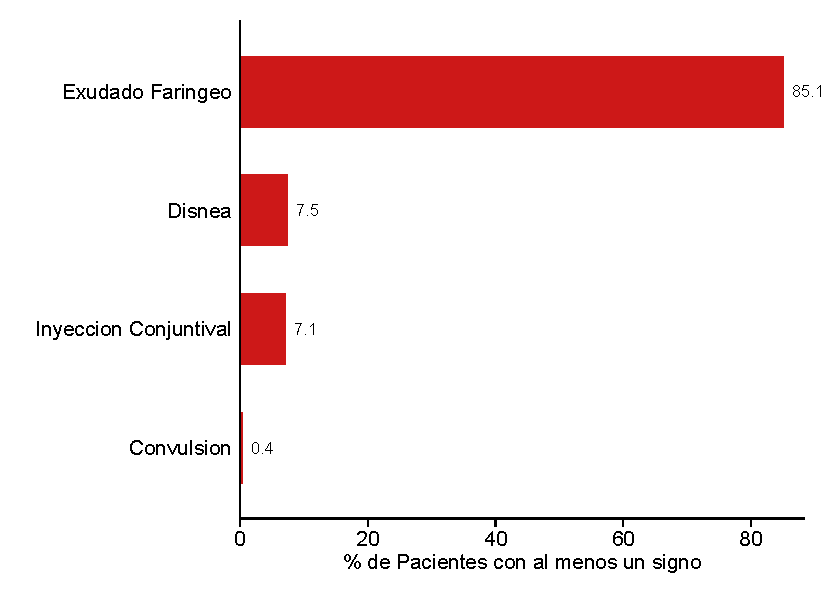
\includegraphics[width=0.65\linewidth]{../figuras/figura_signo.pdf}
	\end{center}
	{\footnotesize {Fuente de datos: NOTICOVID.}}
\end{figure}

La Figura \ref{fig:comorbilidades} muestra la frecuencia de comorbilidades autoreportadas por los pacientes con COVID-19, siendo las más prevalentes la obesidad (31,7 $\%$), diabetes (25,2$\%$) y las comorbilidades cardiovasculares (17,5$\%$).  
\begin{figure}[h]
	\caption{Comorbilidades más frecuentes de los pacientes diagnosticados por COVID-19 en la Región Cusco hasta la SE 07-2022. }\label{fig:comorbilidades}
	\begin{center}
		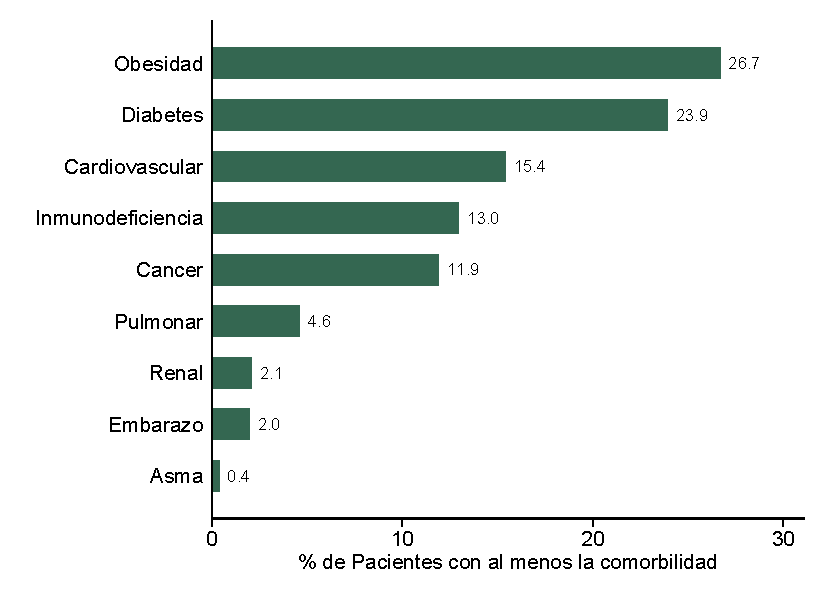
\includegraphics[width=0.65\linewidth]{../figuras/figura_comorbilidad.pdf}
	\end{center}
	{\footnotesize {Fuente de datos: NOTICOVID.}}
\end{figure}
\clearpage
 En la Figura \ref{fig:sintomaticos_asintomati} se evidencia la curva epidémica de casos sintomáticos y asintomáticos, comparada con los casos sintomáticos y asintomáticos desde el año 2020. Desde la SE 04 se evidencia una tendencia marcada al descenso de casos tanto asintomáticos como sintomáticos. 
 
\begin{figure}[h]
	\caption{Casos Sintomáticos y Asintomáticos de COVID-19 por Semana Epidemiológica en la Región Cusco, hasta la SE 07-2022.  }\label{fig:sintomaticos_asintomati}
	
	\begin{center}
		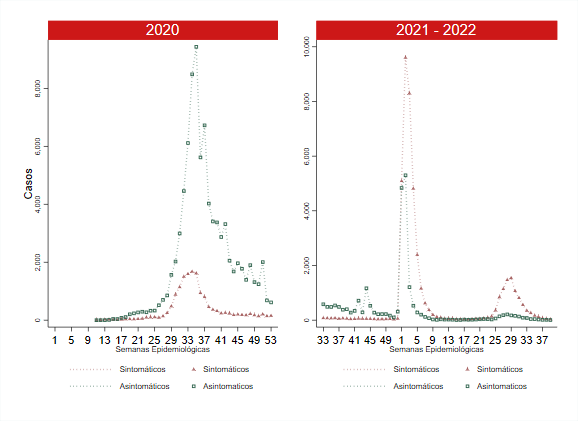
\includegraphics[width=0.75\linewidth]{../figuras/sintomaticos_20_21_22.png}
	\end{center}
	{\footnotesize {Fuente de datos: SISCOVID, NOTICOVID.}}
\end{figure}
\clearpage


%---------------------------------------------------------------------------
% CAPÍTULO: ANÁLISIS DE INDICADORES
%---------------------------------------------------------------------------
%insertar el cover del capitulo
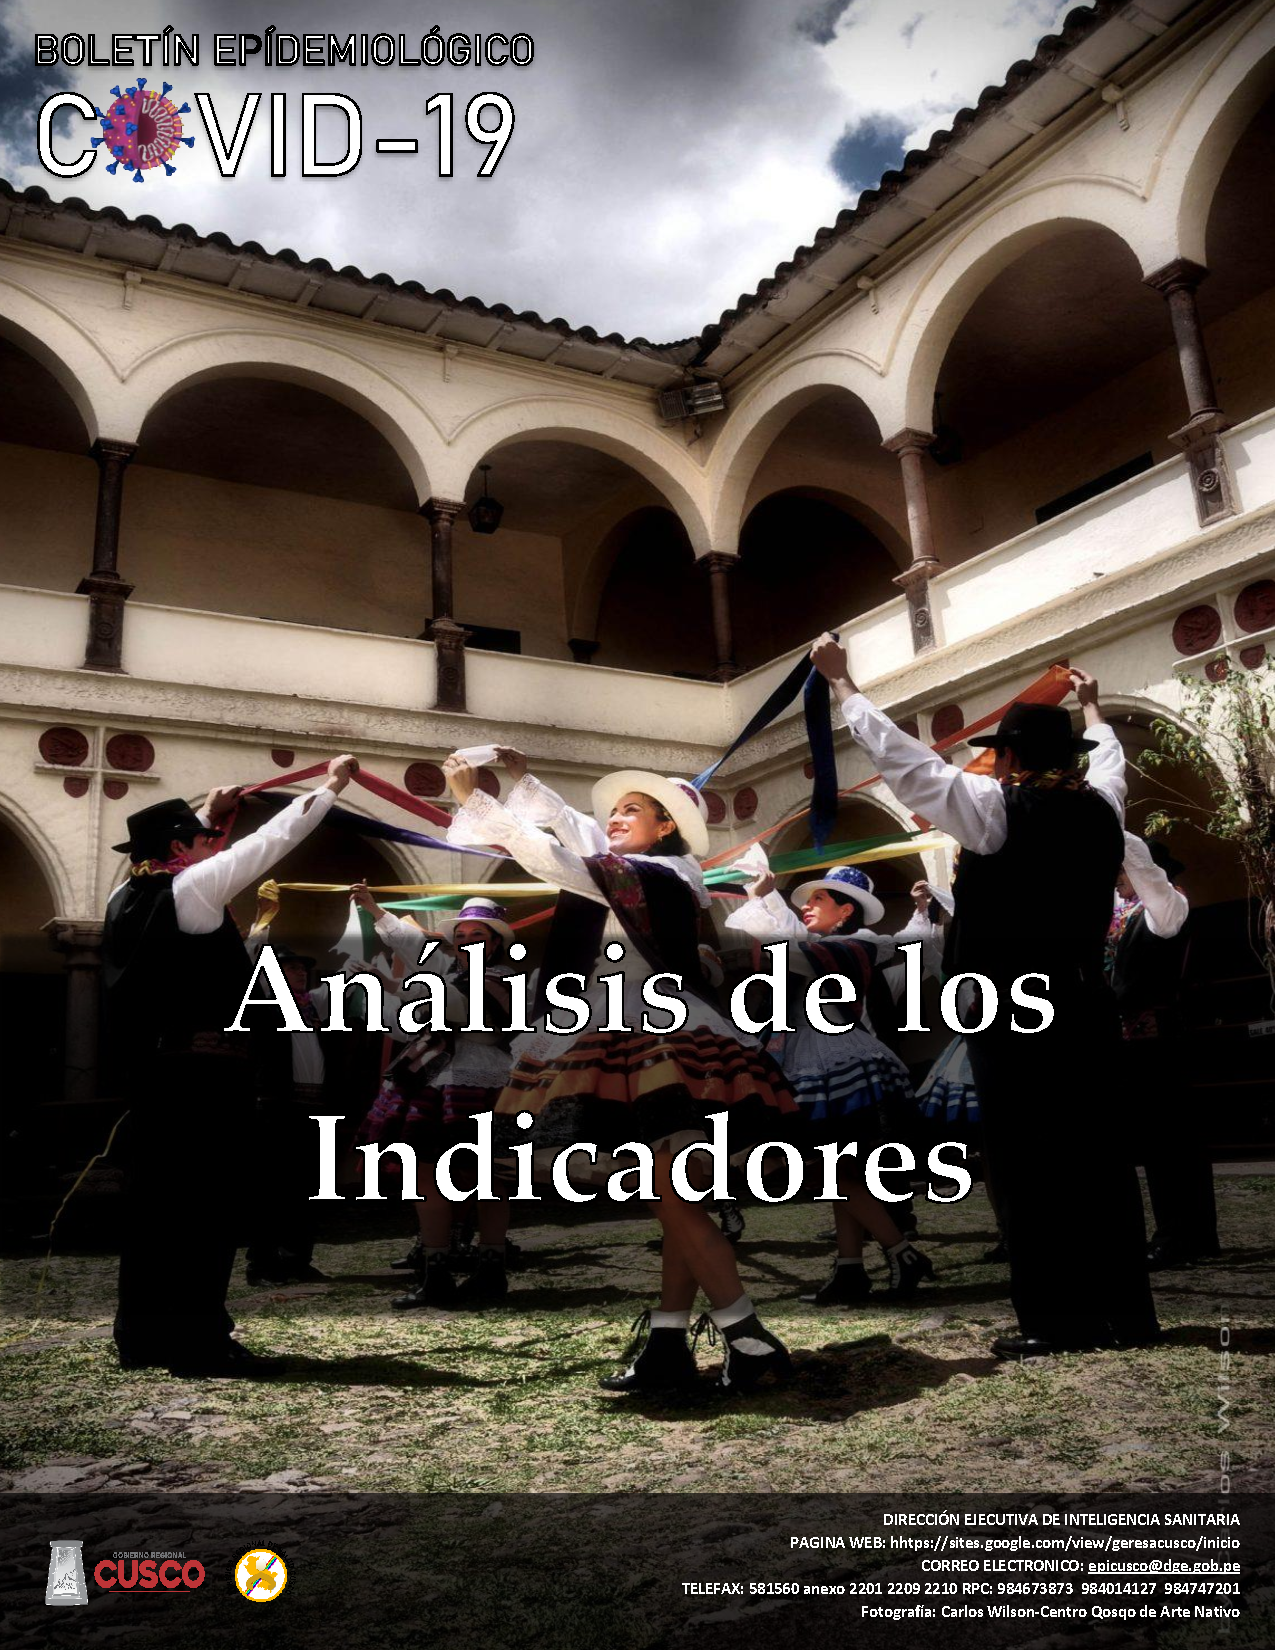
\includepdf[pages={1}]{../editorial/4.pdf}
\clearpage

    \section*{Análisis de Indicadores}
    \addcontentsline{toc}{chapter}{Análisis de Indicadores}
   	\subsection*{Tasa de Incidencia y Tasa de Positividad}
\noindent La evolución de la tasa de incidencia en el tiempo se encuentra graficada en la Figura \ref{fig:incidencia}, tras alcanzar su valor máximo en la SE 03 (1667 casos/1 000 000 personas), hito que marcó el pico de la tercera ola pandémica, la pendiente de la tasa de incidencia se muestra francamente en descenso. Para la SE 07 la tasa de incidencia es del 89 casos/ 1 000 000 personas.  

  \begin{figure}[h]
  	\caption{Tasa de Incidencia de COVID-19 en la región Cusco hasta la SE 07-2022(*).  }\label{fig:incidencia}
  	\begin{center}
  		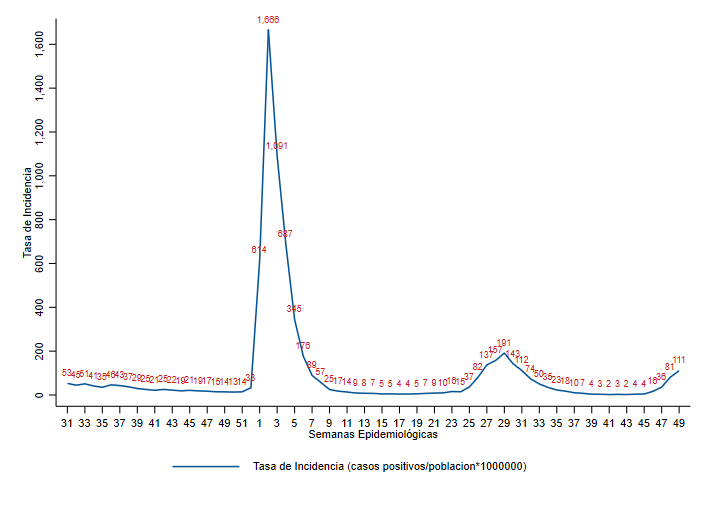
\includegraphics[width=0.80\linewidth]{../figuras/tasa_incidencia_2021_2022.png}
  	\end{center}
  	{\footnotesize {Fuente de datos: SISCOVID, NOTICOVID. (*) Se considera como caso positivo sólo a los pacientes con prueba molecular o antigénica positiva.}}
  \end{figure}
   
  La Figura \ref{fig:total_muestras_procesada} muestra un comparativo de las tasas de positividad ($\%$) de pruebas moleculares (PCR) y antigénicas (AG). En el caso de las muestras PCR, se alcanzó su máximo valor (67$\%$) en la SE 02, tras lo cuál empezó a descender marcadamente. En el caso de la pruebas AG su pico máximo (44$\%$) se alcanzó en la SE 05 posteriormente las cifras reportadas fueron menores semana tras semana.  
  
   \begin{figure}[h]
	\caption{Tasa de positividad para muestras antigénicas y moleculares por COVID-19 en la región Cusco hasta la SE 07-2022. }\label{fig:total_muestras_procesada}
	\begin{center}
		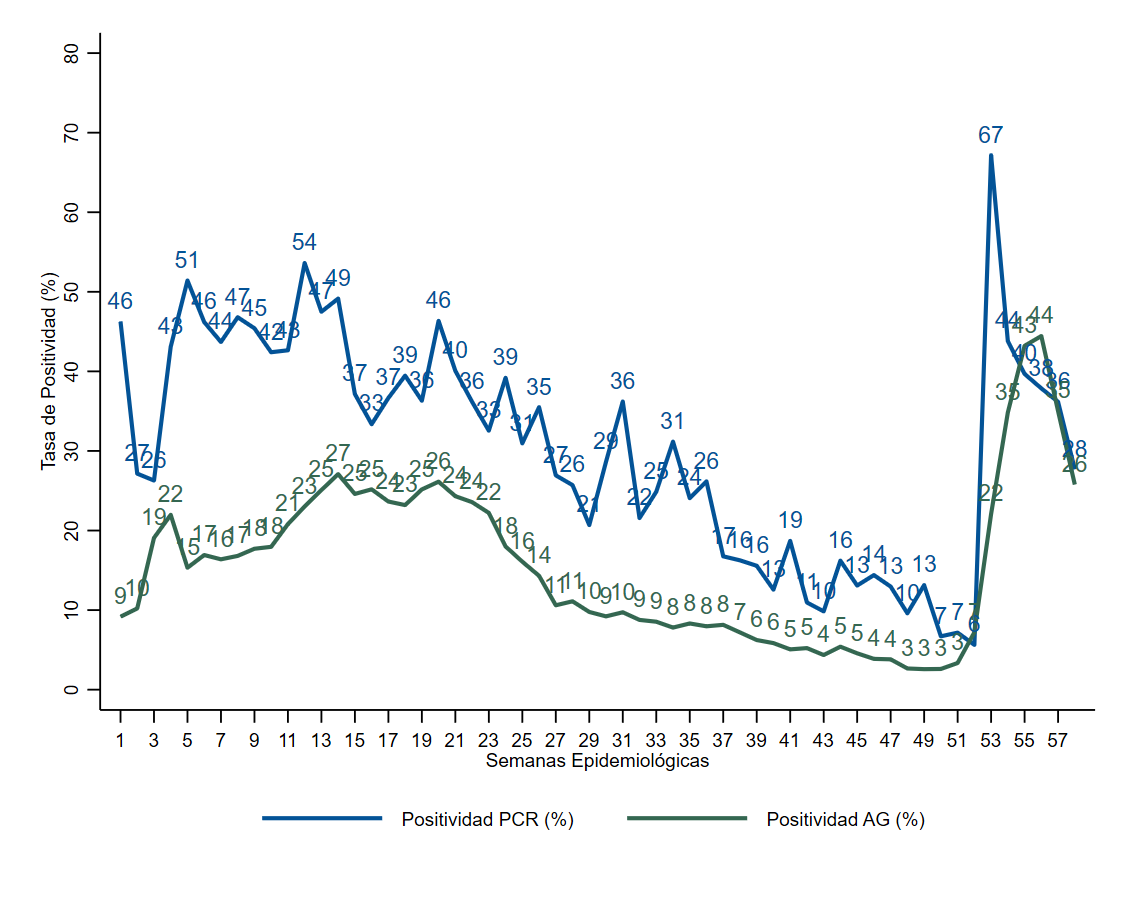
\includegraphics[width=0.75\linewidth]{../figuras/positividad_diaria_2021_2022.png}
	\end{center}
	{\footnotesize {Fuente de datos: SISCOVID, NOTICOVID.}}
\end{figure}


La Figura \ref{fig:positividad_pcr} muestra el número de positivos detectados por pruebas moleculares y su tasa de positividad, se observa que ambos indicadores presentan una tendencia al descenso desde la SE 04 tanto para pruebas moleculares como antigénicas. (Figura \ref{fig:positividad_ag}). 


\begin{landscape}
	\begin{figure}[h]
		\caption{Positividad y Tasa de Positividad de pruebas moleculares tomadas por COVID-19 en la región Cusco hasta la SE 07-2022.}\label{fig:positividad_pcr}
		\begin{center}
			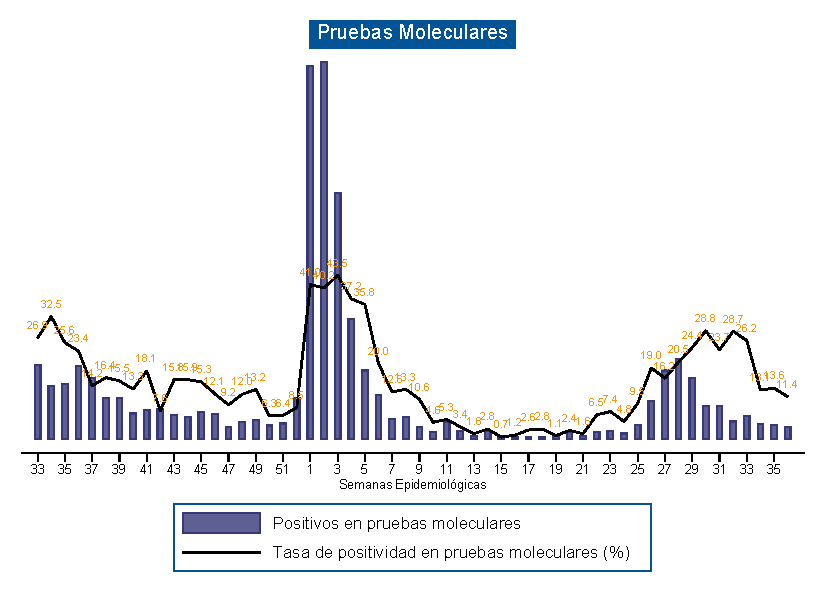
\includegraphics[width=0.90\linewidth]{../figuras/positividad_pcr.pdf}
		\end{center}
		{\footnotesize {Fuente de datos: SISCOVID, NOTICOVID.}}
	\end{figure}
\end{landscape}
\clearpage
\begin{landscape}

	\begin{figure}[h]
		\caption{ Positividad y Tasa de Positividad de pruebas antigénicas tomadas por COVID-19 en la región Cusco hasta la SE 07-2022.}\label{fig:positividad_ag}
		\begin{center}
			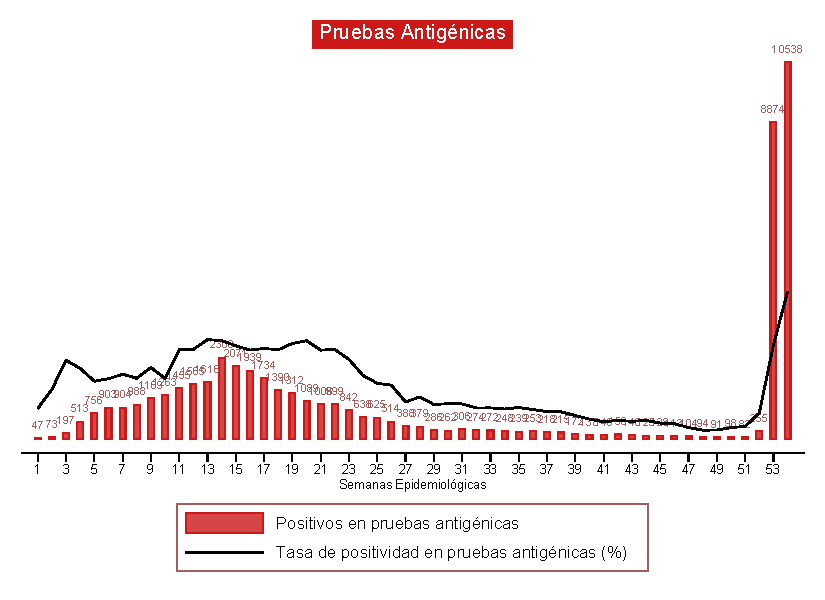
\includegraphics[width=0.90\linewidth]{../figuras/positividad_ag.pdf}
		\end{center}
		{\footnotesize {Fuente de datos: SISCOVID, NOTICOVID.}}
	\end{figure}
\end{landscape}
\clearpage
\subsection*{Análisis de Indicadores en población pediátrica}
\noindent Las figuras inferiores (Figura \ref{fig:niños_2021} y Figura \ref{fig:niño_2022} ) muestran el número de casos positivos(barras rosadas) y número de muertes (línea negra) en la población pediátrica para los quinquenios respectivos.

Para el año 2020 el mayor número de casos positivos en niños se reportó en la SE 35 tras lo cuál el número de casos se ha mantenido variable en el resto del año. Con respecto a las defunciones,  el número máximo de muertes reportada fue de 1 por semana en cada grupo etario. 

En el año 2021 el número de casos positivos se ha mantenido mas o menos constante a lo largo del año hasta la SE 52, tras lo cual se incrementa exponencialmente en todos los quinquenios. Del mismo modo el número de muertes no excedió de 1 muerte por semana en los tres grupos etarios.  

Finalmente para el año 2022 se evidencia un incremento considerable en el número de casos en las primeras semanas distando considerablemente del máximo reportado en las semanas homónimas de los años pasados, incremento que también es acorde al de los otros grupos etarios. Con respecto al número de muertes, el mayor número de muertes reportadas fue de 2 por semana en el quinquenio de 0 a 5 años (Semana epidemiológica 07). 


En la Figura \ref{fig:letalidad_niños} se evidencia el número de casos positivos, las defunciones y la tasa de letalidad de menores de 15 años, agrupados por quinquenios. Se evidencia que hasta la SE 07 del año 2022 se reportaron 2420 casos positivos y 6 defunciones en este grupo etario, teniendo una letalidad de 0,25 $\%$, porcentaje que aún es menor a las primeras olas de afección por COVID-19  

\begin{figure}[h]
	\caption{Casos y defunciones por quinquenio en población pediátrica 2020-2021.}
	\label{fig:niños_2021}
	\centering
	\begin{subfigure}[b]{0.45\textwidth}
		\centering
		\includegraphics[width=\textwidth]{../figuras/niños_2020_1.pdf}
		\caption{De 0 a 5 años - \textbf{2020}}
		%\label{fig:}
	\end{subfigure}
	\hfill
	\begin{subfigure}[b]{0.45\textwidth}
		\centering
		\includegraphics[width=\textwidth]{../figuras/niños_2021_1.pdf}
		\caption{De 0 a 5 años - \textbf{2021}}
		%\label{fig:70 a 79 años}
	\end{subfigure}
	
	\vspace{10mm}
	\begin{subfigure}[b]{0.45\textwidth}
		\centering
		\includegraphics[width=\textwidth]{../figuras/niños_2020_2.pdf}
		\caption{De 6 a 11 años - \textbf{2020}}
		%\label{fig:60 a 69 años}
	\end{subfigure}
	\hfill
	\begin{subfigure}[b]{0.45\textwidth}
		\centering
		\includegraphics[width=\textwidth]{../figuras/niños_2021_2.pdf}
		\caption{De 6 a 10 años - \textbf{2021}}
		%\label{fig:50 a 59 años}
	\end{subfigure}
	
	\vspace{10mm}
	\begin{subfigure}[b]{0.45\textwidth}
		\centering
		\includegraphics[width=\textwidth]{../figuras/niños_2020_3.pdf}
		\caption{De 11 a 15 años - \textbf{2020}}
		%\label{fig:40 a 49 años}
	\end{subfigure}
	\hfill
	\begin{subfigure}[b]{0.45\textwidth}
		\centering
		\includegraphics[width=\textwidth]{../figuras/niños_2021_3.pdf}
		\caption{De 11 a 15 años - \textbf{2021}}
		%\label{fig:40 a 49 años}
	\end{subfigure}
\end{figure}

\begin{figure}[h]
	\caption{Casos y defunciones por quinquenio en población pediátrica - 2022.}
	\label{fig:niño_2022}
	\centering
	\begin{subfigure}[b]{0.45\textwidth}
		\centering
		\includegraphics[width=\textwidth]{../figuras/niños_2022_1.pdf}
		\caption{De 0 a 5 años - \textbf{2022}}
		%\label{fig:40 a 49 años}
	\end{subfigure}
	
	\centering
	\begin{subfigure}[b]{0.45\textwidth}
		\centering
		\includegraphics[width=\textwidth]{../figuras/niños_2022_2.pdf}
		\caption{De 6 a 10 años - \textbf{2022}}
		%\label{fig:40 a 49 años}
	\end{subfigure}
	
	\vspace{10mm}
	\begin{subfigure}[b]{0.45\textwidth}
		\centering
		\includegraphics[width=\textwidth]{../figuras/niños_2022_3.pdf}
		\caption{De 11 a 15 años - \textbf{2022}}
		%\label{fig:40 a 49 años}
	\end{subfigure}
\end{figure}

	\begin{table}[]
		\resizebox{\textwidth}{!}{%
				\begin{tabular}{lcccc}
		\cline{2-5}
		\multicolumn{1}{l|}{} &
		\multicolumn{1}{c|}{\cellcolor[HTML]{ECF4FF}Etapa de Vida} &
		\multicolumn{1}{c|}{\cellcolor[HTML]{ECF4FF}Positivos} &
		\multicolumn{1}{c|}{\cellcolor[HTML]{ECF4FF}Defunciones} &
		\multicolumn{1}{c|}{\cellcolor[HTML]{ECF4FF}Letalidad(\%)} \\ \hline
		\multicolumn{1}{|l|}{} &
		\multicolumn{1}{c|}{0 a 5 años} &
		\multicolumn{1}{c|}{851} &
		\multicolumn{1}{c|}{4} &
		\multicolumn{1}{c|}{0.47} \\ \cline{2-5} 
		\multicolumn{1}{|l|}{} &
		\multicolumn{1}{c|}{6 a 10 años} &
		\multicolumn{1}{c|}{705} &
		\multicolumn{1}{c|}{2} &
		\multicolumn{1}{c|}{0.28} \\ \cline{2-5} 
		\multicolumn{1}{|l|}{} &
		\multicolumn{1}{c|}{11 a 15 años} &
		\multicolumn{1}{c|}{1146} &
		\multicolumn{1}{c|}{2} &
		\multicolumn{1}{c|}{0.17} \\ \cline{2-5} 
		\multicolumn{1}{|l|}{\multirow{-4}{*}{2020}} &
		\multicolumn{1}{c|}{\cellcolor[HTML]{ECF4FF}Total} &
		\multicolumn{1}{c|}{\cellcolor[HTML]{ECF4FF}2702} &
		\multicolumn{1}{c|}{\cellcolor[HTML]{ECF4FF}8} &
		\multicolumn{1}{c|}{\cellcolor[HTML]{ECF4FF}0.30} \\ \hline
		&
		\multicolumn{1}{l}{} &
		\multicolumn{1}{l}{} &
		\multicolumn{1}{l}{} &
		\multicolumn{1}{l}{} \\ \cline{2-5} 
		\multicolumn{1}{l|}{} &
		\multicolumn{1}{c|}{\cellcolor[HTML]{ECF4FF}Etapa de Vida} &
		\multicolumn{1}{c|}{\cellcolor[HTML]{ECF4FF}Positivos} &
		\multicolumn{1}{c|}{\cellcolor[HTML]{ECF4FF}Defunciones} &
		\multicolumn{1}{c|}{\cellcolor[HTML]{ECF4FF}Letalidad(\%)} \\ \hline
		\multicolumn{1}{|l|}{} &
		\multicolumn{1}{c|}{0 a 5 años} &
		\multicolumn{1}{c|}{517} &
		\multicolumn{1}{c|}{7} &
		\multicolumn{1}{c|}{1.4} \\ \cline{2-5} 
		\multicolumn{1}{|l|}{} &
		\multicolumn{1}{c|}{6 a 10 años} &
		\multicolumn{1}{c|}{484} &
		\multicolumn{1}{c|}{4} &
		\multicolumn{1}{c|}{0.83} \\ \cline{2-5} 
		\multicolumn{1}{|l|}{} &
		\multicolumn{1}{c|}{11 a 15 años} &
		\multicolumn{1}{c|}{1284} &
		\multicolumn{1}{c|}{3} &
		\multicolumn{1}{c|}{0.23} \\ \cline{2-5} 
		\multicolumn{1}{|l|}{\multirow{-4}{*}{2021}} &
		\multicolumn{1}{c|}{\cellcolor[HTML]{ECF4FF}Total} &
		\multicolumn{1}{c|}{\cellcolor[HTML]{ECF4FF}2285} &
		\multicolumn{1}{c|}{\cellcolor[HTML]{ECF4FF}14} &
		\multicolumn{1}{c|}{\cellcolor[HTML]{ECF4FF}0.61} \\ \hline
		&
		\multicolumn{1}{l}{} &
		\multicolumn{1}{l}{} &
		\multicolumn{1}{l}{} &
		\multicolumn{1}{l}{} \\ \cline{2-5} 
		\multicolumn{1}{l|}{} &
		\multicolumn{1}{c|}{\cellcolor[HTML]{ECF4FF}Etapa de Vida} &
		\multicolumn{1}{c|}{\cellcolor[HTML]{ECF4FF}Positivos} &
		\multicolumn{1}{c|}{\cellcolor[HTML]{ECF4FF}Defunciones} &
		\multicolumn{1}{c|}{\cellcolor[HTML]{ECF4FF}Letalidad(\%)} \\ \hline
		\multicolumn{1}{|l|}{} &
		\multicolumn{1}{c|}{0 a 5 años} &
		\multicolumn{1}{c|}{604} &
		\multicolumn{1}{c|}{5} &
		\multicolumn{1}{c|}{0.83} \\ \cline{2-5} 
		\multicolumn{1}{|l|}{} &
		\multicolumn{1}{c|}{6 a 10 años} &
		\multicolumn{1}{c|}{720} &
		\multicolumn{1}{c|}{1} &
		\multicolumn{1}{c|}{0.14} \\ \cline{2-5} 
		\multicolumn{1}{|l|}{} &
		\multicolumn{1}{c|}{11 a 15 años} &
		\multicolumn{1}{c|}{1096} &
		\multicolumn{1}{c|}{0} &
		\multicolumn{1}{c|}{0} \\ \cline{2-5} 
		\multicolumn{1}{|l|}{\multirow{-4}{*}{2022}} &
		\multicolumn{1}{c|}{\cellcolor[HTML]{ECF4FF}Total} &
		\multicolumn{1}{c|}{\cellcolor[HTML]{ECF4FF}2420} &
		\multicolumn{1}{c|}{\cellcolor[HTML]{ECF4FF}6} &
		\multicolumn{1}{c|}{\cellcolor[HTML]{ECF4FF}0.25} \\ \hline
	\end{tabular}
		}
	\end{table}	
\clearpage

	\subsection*{Análisis de la Mortalidad}

\noindent En la Figura \ref{fig:mortalidad_edad} se muestra la mortalidad semanal para las edades agrupadas en decenios, se evidencia el ascenso de la curva de mortalidad hasta la SE 05 a expensas de las muertes reportadas en el grupo etario de mayores 80 años, luego de ello la tasa de mortalidad presenta una pendiente en descenso. Es importante recalcar que el pico de muertes reportados en esta ola dista bastante del pico reportado en la segunda ola y primera ola, donde la mortalidad fue mucho mayor.  
	 	
\begin{figure}[h]
	\caption{Tasa de Mortalidad por COVID-19 por Grupo Etario hasta la SE 07-2022.}\label{fig:mortalidad_edad}
	\begin{center}
		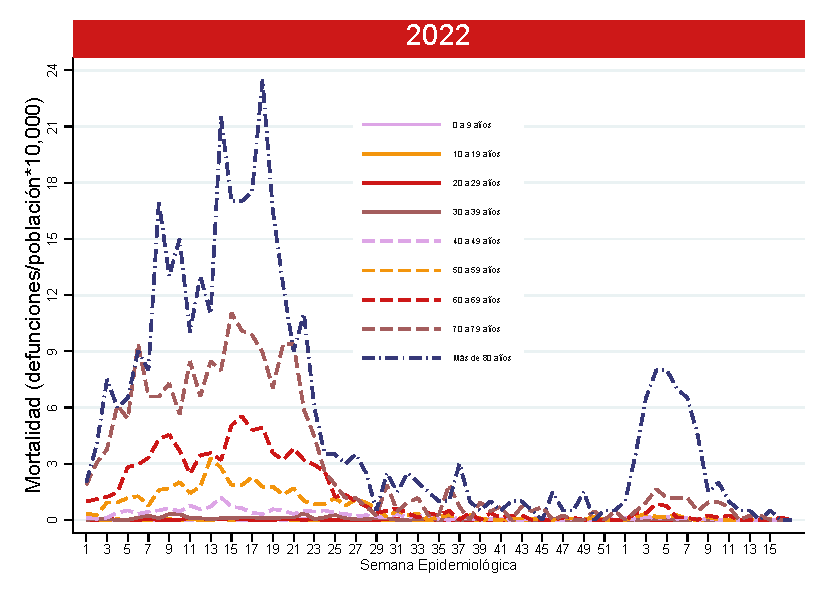
\includegraphics[width=0.65\linewidth]{../figuras/mortalidad_edad_2021_2022.pdf}
	\end{center}
	{\footnotesize Fuente de datos: SINADEF} 
\end{figure}


La Figura \ref{fig:mortalidad_grupo_edad} muestra la relación entre la tasa de mortalidad y la vacunación en todos los grupos etarios. Las líneas de referencia rojas representan las fechas del inicio de la vacunación (primera dosis) para el correspondiente grupo etario y la linea verde el inicio de la tercera ola pandémica. Se observa que tras el inicio de la tercera ola se han reportado muertes en todos los grupos etarios, generando una pendiente en ascenso de la tasa de mortalidad hasta la SE 07. Sin embargo, en los grupos donde la inmunización comenzó el año 2021 estas cifras distan bastante de las máximas reportadas en la segunda ola. En el caso de grupo etario de 0 a 9 años, se aprecia que la vacunación inició la SE 04 del 2022 por lo cuál aún no es evidente el efecto de la vacunación en la tasa de mortalidad. 

	\begin{figure}[h]
	\caption{Tasa de Mortalidad por COVID-19 por Grupo Etario hasta la SE 07-2022.}
	\label{fig:mortalidad_grupo_edad}
	\centering
	\begin{subfigure}[b]{0.45\textwidth}
		\centering
		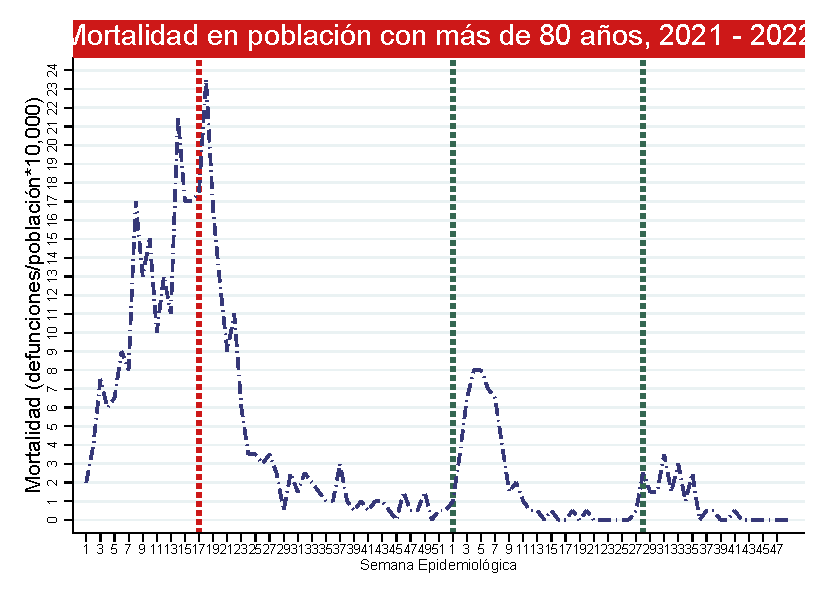
\includegraphics[width=\textwidth]{../figuras/mortalidad_edad_80.pdf}
		\caption{Más de 80 años}
		%\label{fig:}
	\end{subfigure}
	\hfill
	\begin{subfigure}[b]{0.45\textwidth}
		\centering
		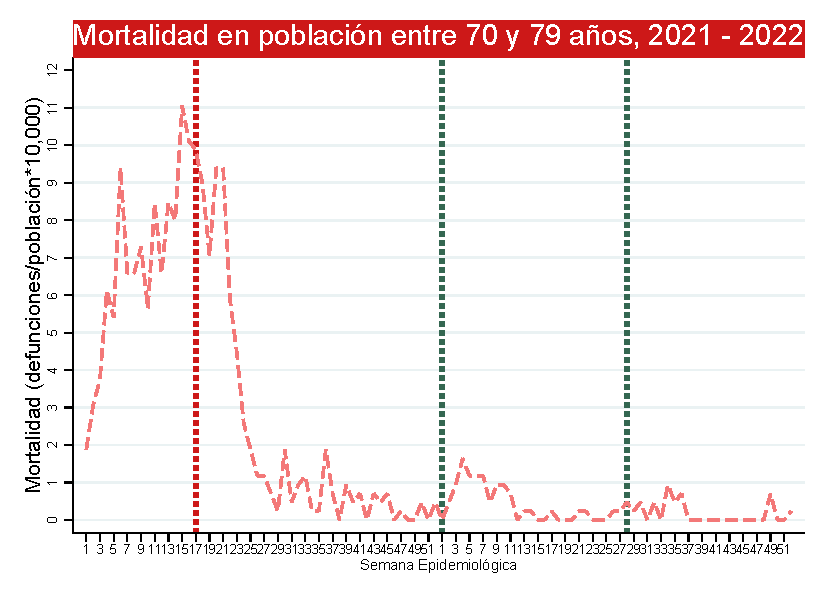
\includegraphics[width=\textwidth]{../figuras/mortalidad_edad_70.pdf}
		\caption{70 a 79 años}
		%\label{fig:70 a 79 años}
	\end{subfigure}

	\vspace{10mm}
	\begin{subfigure}[b]{0.45\textwidth}
		\centering
		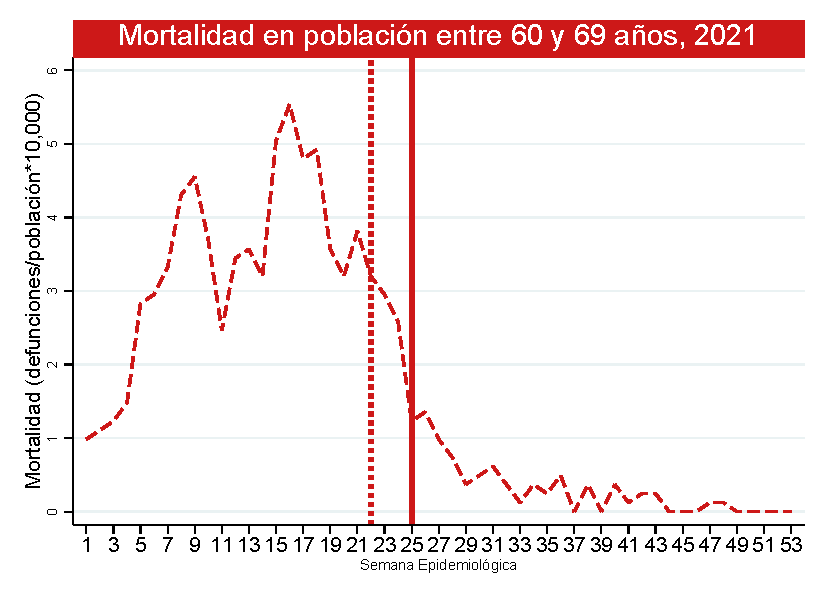
\includegraphics[width=\textwidth]{../figuras/mortalidad_edad_60.pdf}
		\caption{60 a 69 años}
		%\label{fig:60 a 69 años}
	\end{subfigure}
	\hfill
	\begin{subfigure}[b]{0.45\textwidth}
		\centering
		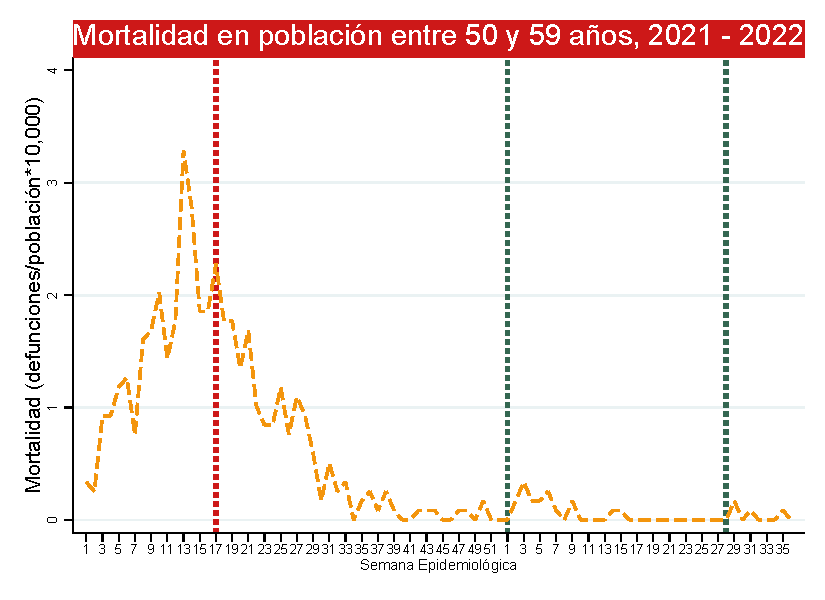
\includegraphics[width=\textwidth]{../figuras/mortalidad_edad_50.pdf}
		\caption{50 a 59 años}
		%\label{fig:50 a 59 años}
	\end{subfigure}

	\vspace{10mm}
	\begin{subfigure}[b]{0.45\textwidth}
		\centering
		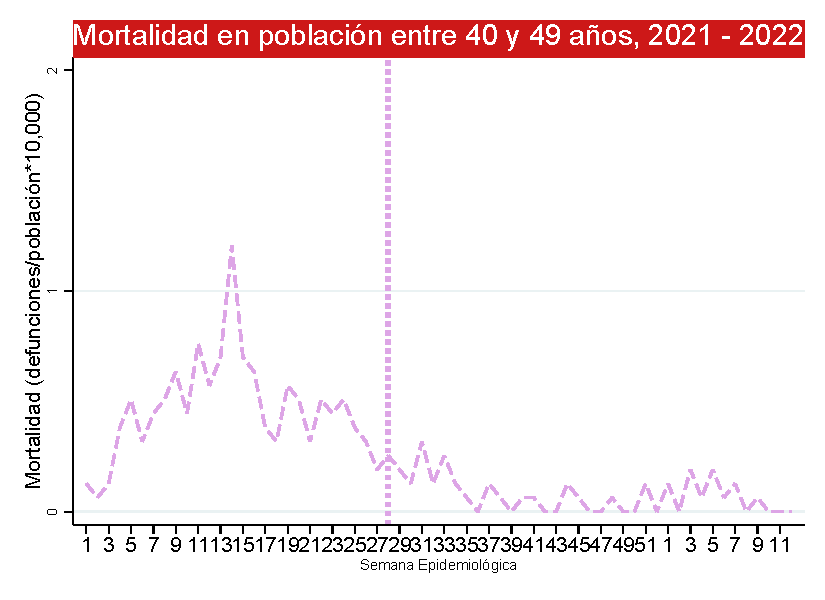
\includegraphics[width=\textwidth]{../figuras/mortalidad_edad_40.pdf}
		\caption{40 a 49 años}
		%\label{fig:40 a 49 años}
	\end{subfigure}
	\hfill
	\begin{subfigure}[b]{0.45\textwidth}
		\centering
		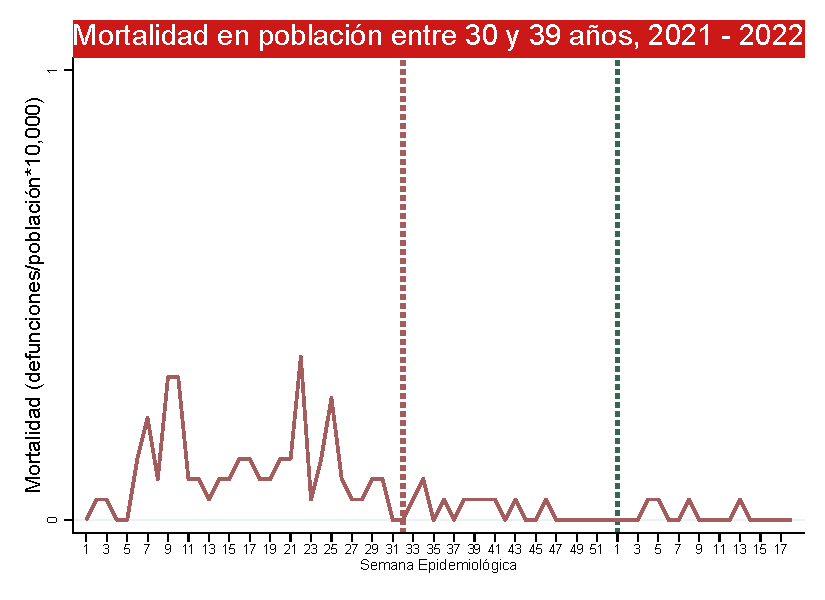
\includegraphics[width=\textwidth]{../figuras/mortalidad_edad_30.pdf}
		\caption{30 a 39 años}
		%\label{fig:40 a 49 años}
	\end{subfigure}
	\end{figure}

	\begin{figure}[h]
	\caption{Tasa de Mortalidad por COVID-19 por Grupo Etario hasta la SE 07-2022.}
	\label{fig:mortalidad_grupo_edad_2}
	\centering
	\begin{subfigure}[b]{0.45\textwidth}
		\centering
		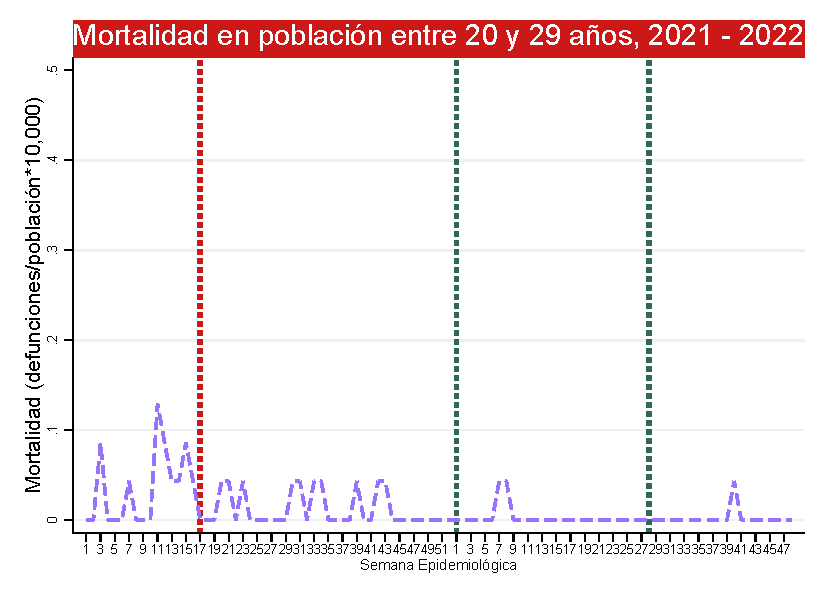
\includegraphics[width=\textwidth]{../figuras/mortalidad_edad_20.pdf}
		\caption{20 a 29 años}
		%\label{fig:40 a 49 años}
	\end{subfigure}

	\centering
	\begin{subfigure}[b]{0.45\textwidth}
		\centering
		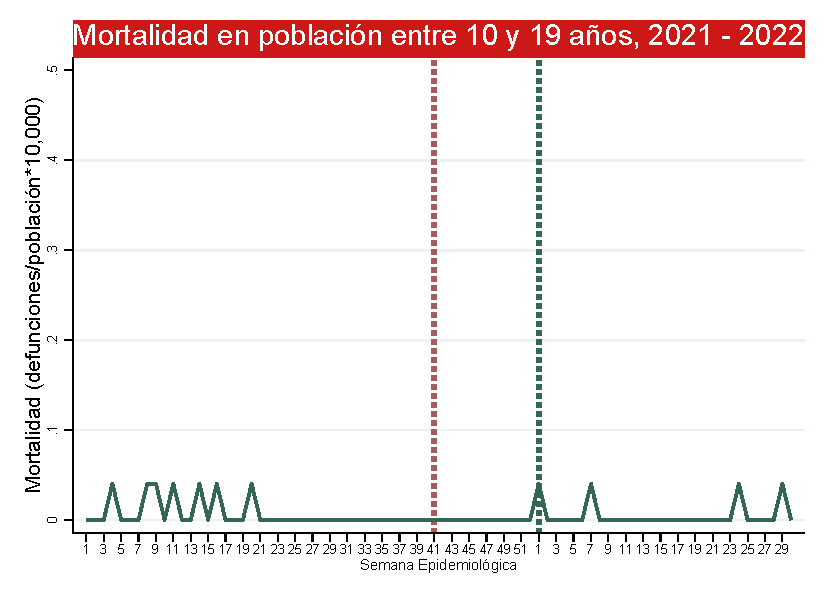
\includegraphics[width=\textwidth]{../figuras/mortalidad_edad_10.pdf}
		\caption{10 a 19 años}
		%\label{fig:40 a 49 años}
	\end{subfigure}
	
	\vspace{10mm}
	\begin{subfigure}[b]{0.45\textwidth}
		\centering
		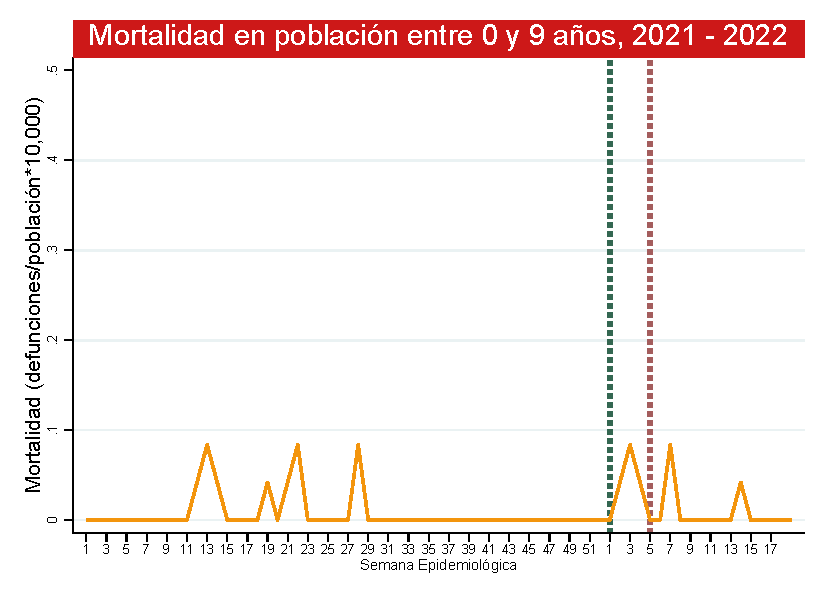
\includegraphics[width=\textwidth]{../figuras/mortalidad_edad_0.pdf}
		\caption{0 a 09 años}
		%\label{fig:40 a 49 años}
	\end{subfigure}
\end{figure}
\clearpage	
	\subsection*{Exceso de Muertes por Todas las Causas}
\noindent La Figura \ref{fig:exceso_regional} muestra la tendencia del exceso de muertes con respecto al año 2019. Se reporta un exceso de 8 defunciones para la SE 07 del 2022.

	\begin{figure}[h]
	\caption{Exceso de Fallecidos por Todas las Causas en la Región Cusco hasta la SE 07-2022.}\label{fig:exceso_regional}
	\begin{center}
		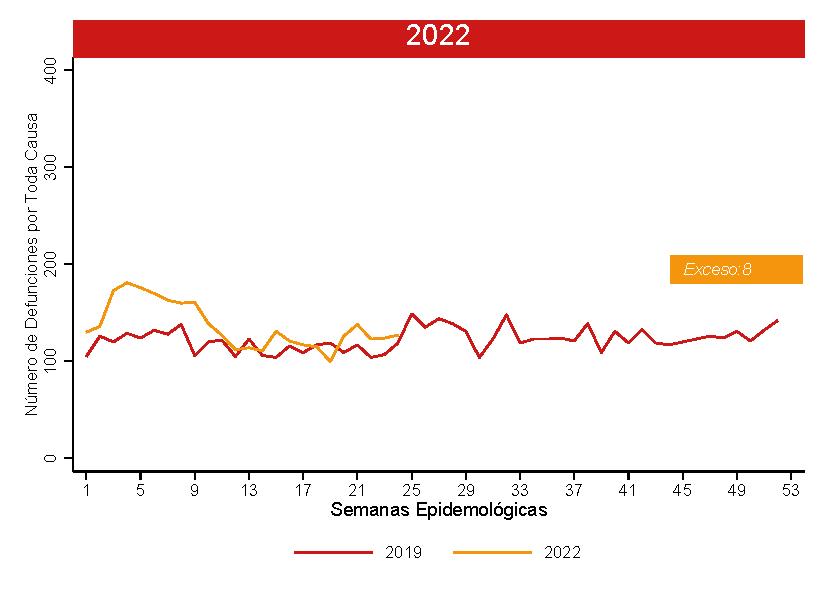
\includegraphics[width=0.85\linewidth]{../figuras/exceso_region_2022.pdf}
	\end{center}
	{\footnotesize {Fuente de datos: SISCOVID, NOTICOVID.}}
	\end{figure}
\clearpage

	\subsection*{Cobertura de Vacunación por COVID-19 en la Región Cusco, hasta la SE 07-2022.}
\noindent La Figura \ref{fig:vacuna_edad} muestra la cobertura de vacunación por grupo etario en la Región Cusco. El grupo etario con mejor cobertura es el de 70 a 79 años con 89,9 $\%$ de la población objetivo con 2 dosis aplicadas, seguido del grupo etario de 60 a 69 años con 88,8 $\%$. Asimismo, se evidencia que el grupo etario de 5 a 11 años, cuya vacunacion comenzó la SE 04, tiene el 2,6 $\%$ de su población con 2 dosis aplicadas.  

\begin{figure}[h]
	\caption{Cobertura de Vacunación por Grupo Etario en la Región Cusco hasta la SE 07-2022. }\label{fig:vacuna_edad}
	\begin{center}
		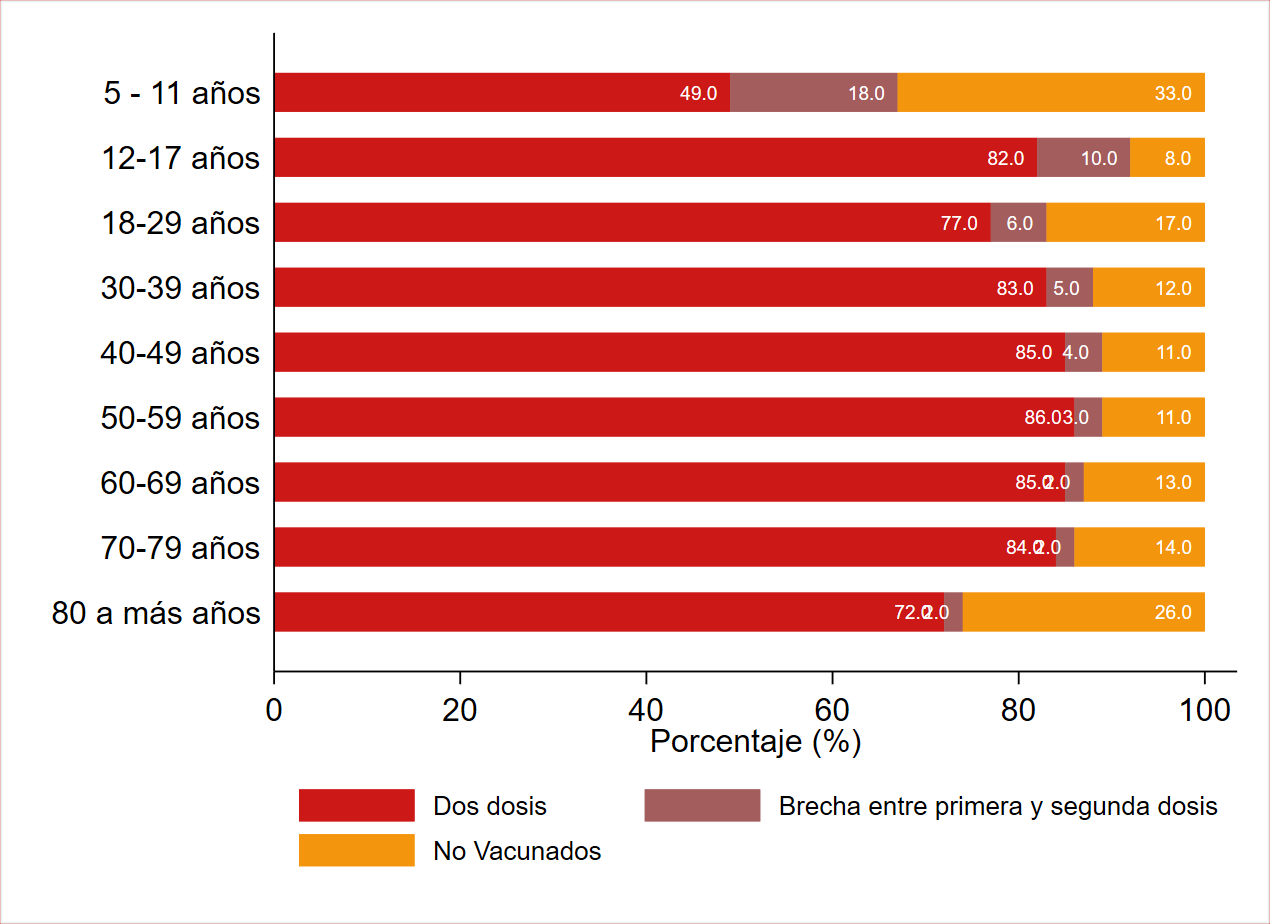
\includegraphics[width=0.90\linewidth]{../figuras/vacunacion_grupo_edad.png}
	\end{center}
	{\footnotesize {Fuente de datos: SICOVAC, HIS-MINSA.}}
\end{figure}

%La Figura \ref{fig:cobertura_vacunaci_provincia}  muestra la cobertura de vacunación en cada una de las provincias de Cusco por grupo etario. Es preciso señalar que la provincia de Espinar tiene la cobertura más baja de la región, en los grupos etarios desde los 50 años en adelante.
%
%\begin{figure}[h]
%	\caption{Cobertura de Vacunación por Provincia y por Grupo Etario en la Región Cusco, hasta la SE 51.}
%	\label{fig:cobertura_vacunaci_provincia}
%	\centering
%	\begin{subfigure}[b]{0.45\textwidth}
%		\centering
%		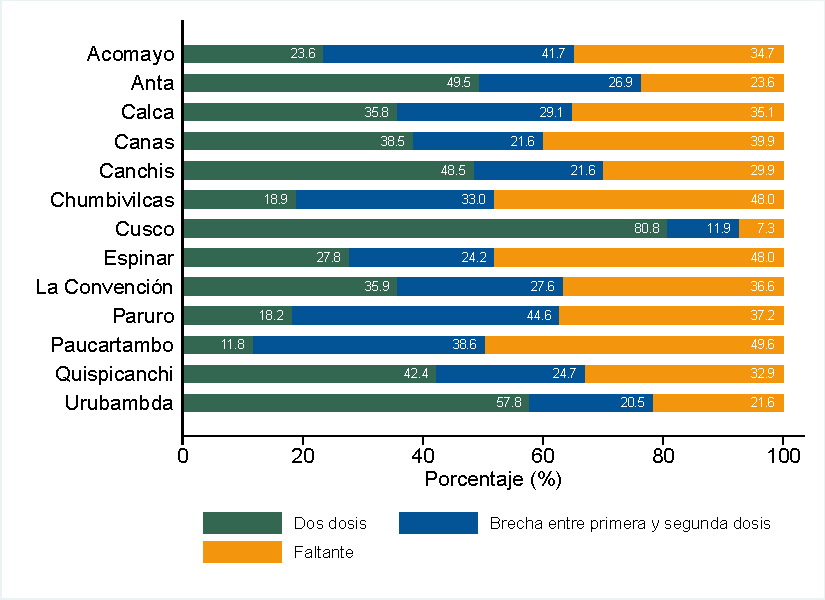
\includegraphics[width=\textwidth]{../figuras/vacunacion_provincial_edad_1}
%		\caption{ De 12 a 19 años}
%		%\label{fig:}
%	\end{subfigure}
%	\hfill
%	\begin{subfigure}[b]{0.45\textwidth}
%		\centering
%		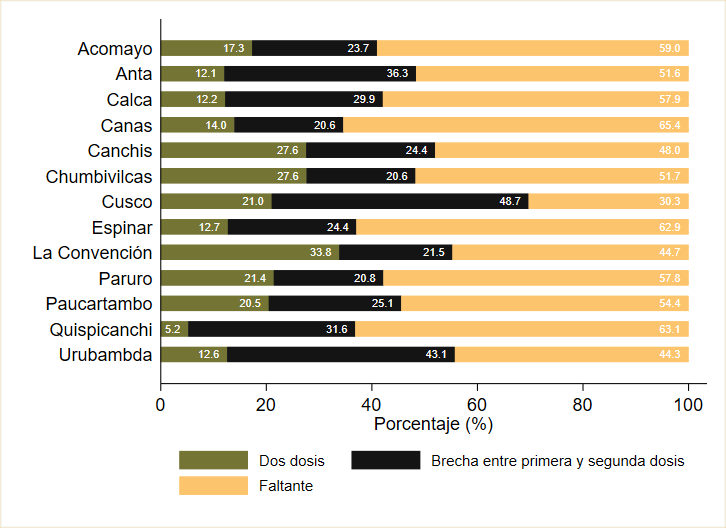
\includegraphics[width=\textwidth]{../figuras/vacunacion_provincial_edad_2}
%		\caption{De 20 a 29 años}
%		%\label{fig:70 a 79 años}
%	\end{subfigure}
%	\begin{subfigure}[b]{0.45\textwidth}
%		\centering
%		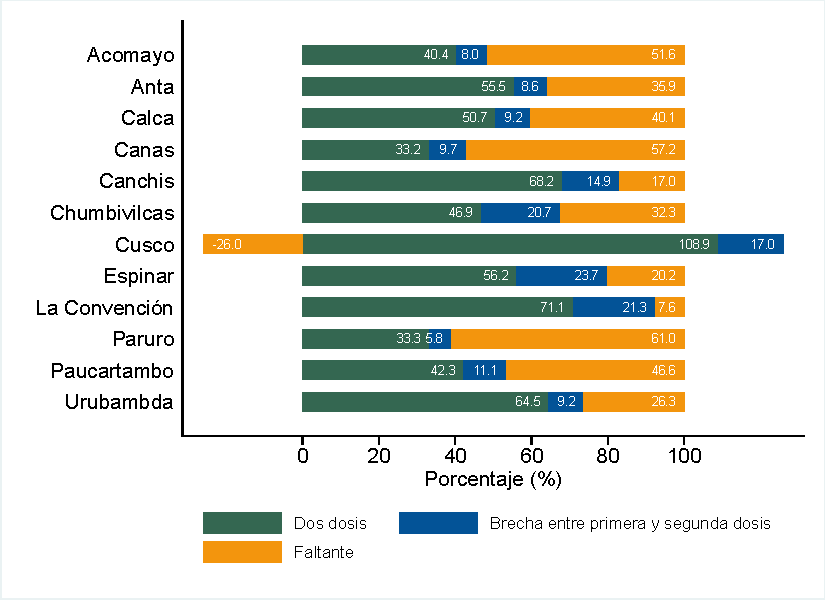
\includegraphics[width=\textwidth]{../figuras/vacunacion_provincial_edad_3}
%		\caption{De 30 a 39 años}
%		%\label{fig:60 a 69 años}
%	\end{subfigure}
%	\hfill
%	\begin{subfigure}[b]{0.45\textwidth}
%		\centering
%		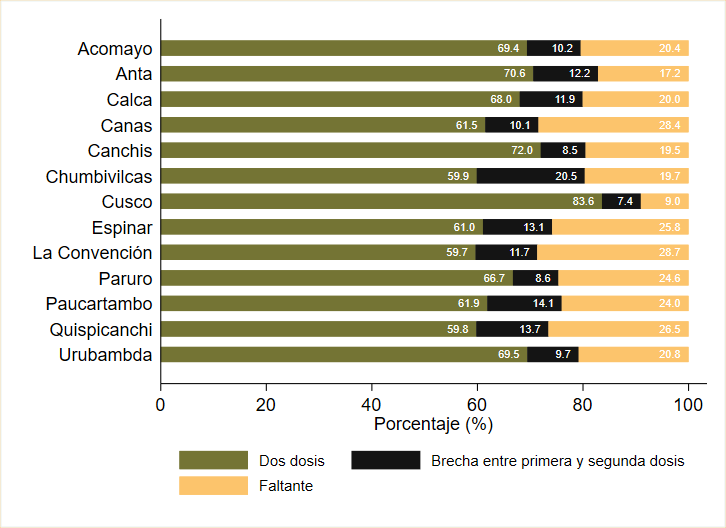
\includegraphics[width=\textwidth]{../figuras/vacunacion_provincial_edad_4}
%		\caption{De 40 a 49 años}
%		%\label{fig:50 a 59 años}
%	\end{subfigure}
%	\begin{subfigure}[b]{0.45\textwidth}
%		\centering
%		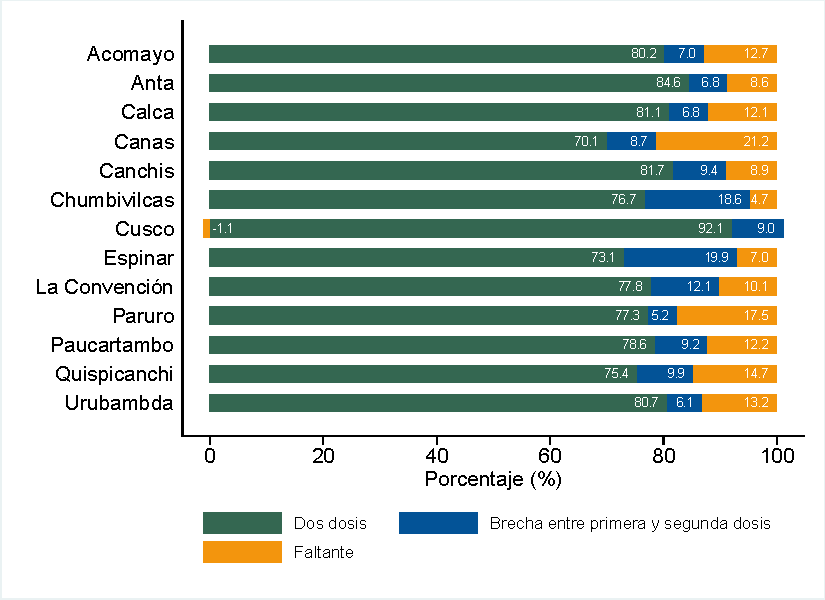
\includegraphics[width=\textwidth]{../figuras/vacunacion_provincial_edad_5}
%		\caption{De 50 a 59 años}
%		%\label{fig:40 a 49 años}
%	\end{subfigure}
%	\hfill
%	\begin{subfigure}[b]{0.45\textwidth}
%		\centering
%		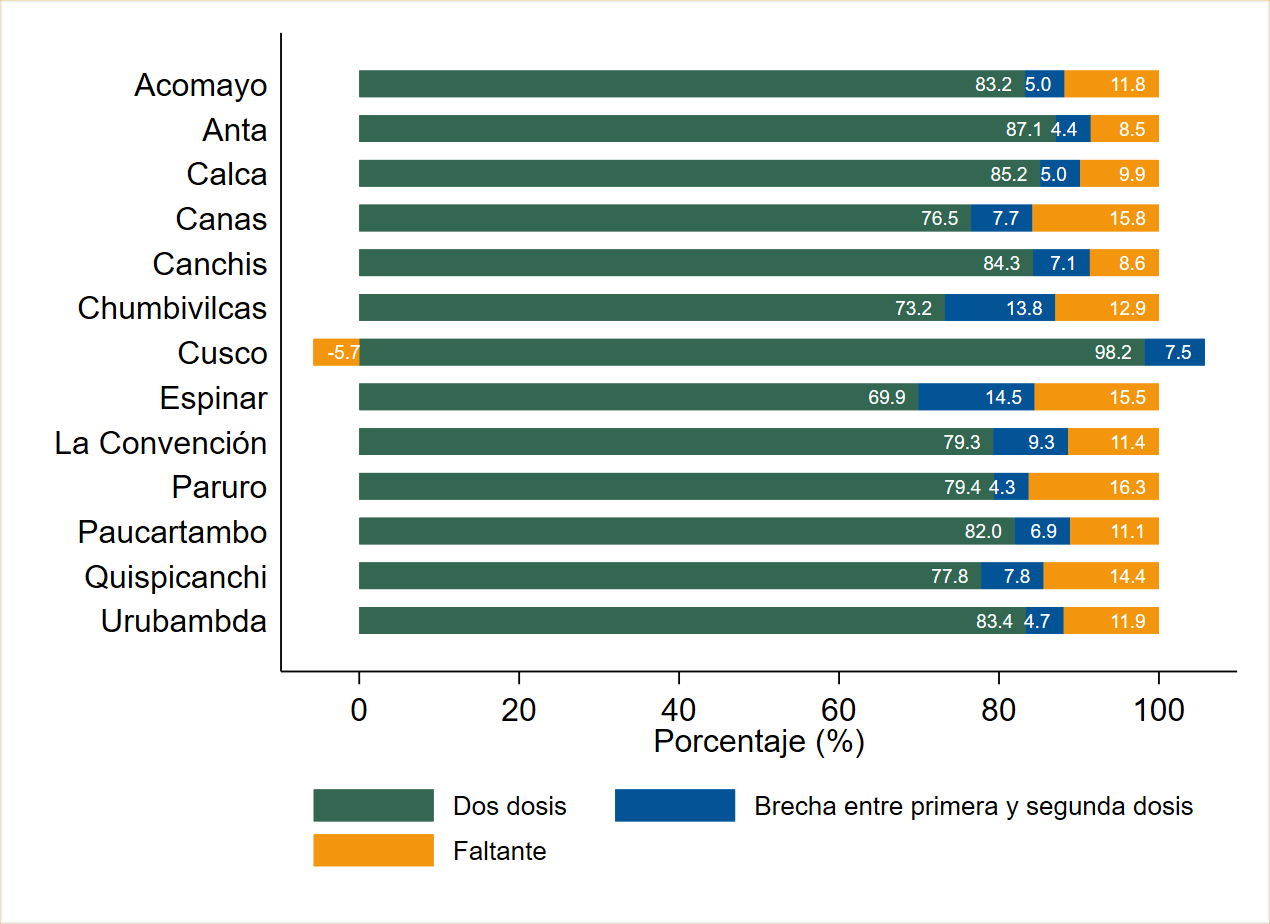
\includegraphics[width=\textwidth]{../figuras/vacunacion_provincial_edad_6}
%		\caption{De 60 a 69 años}
%		%\label{fig:40 a 49 años}
%	\end{subfigure}
%\begin{subfigure}[b]{0.45\textwidth}
%	\centering
%	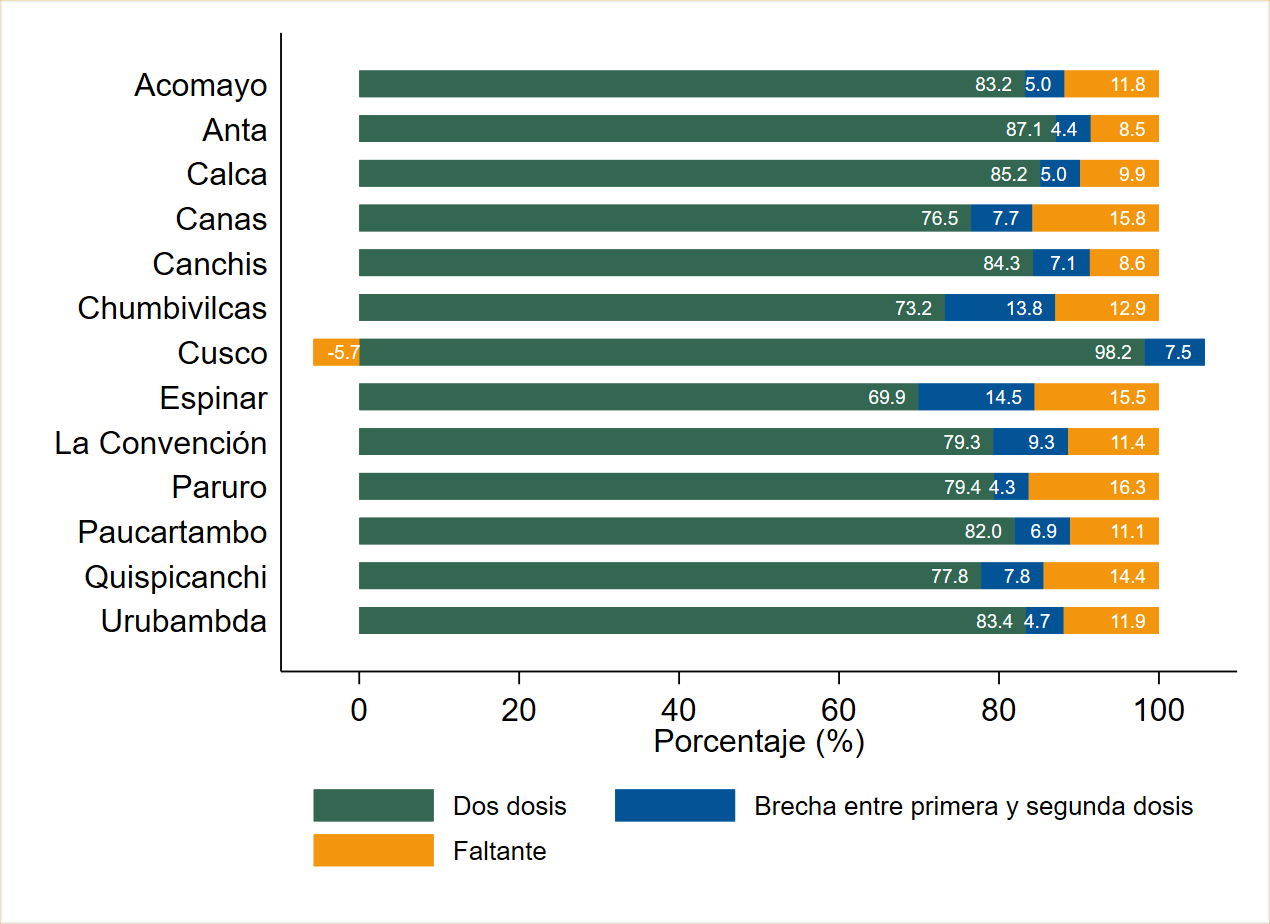
\includegraphics[width=\textwidth]{../figuras/vacunacion_provincial_edad_6}
%	\caption{De 70 a 79 años}
%	%\label{fig:40 a 49 años}
%\end{subfigure}
%\hfill
%\begin{subfigure}[b]{0.45\textwidth}
%	\centering
%	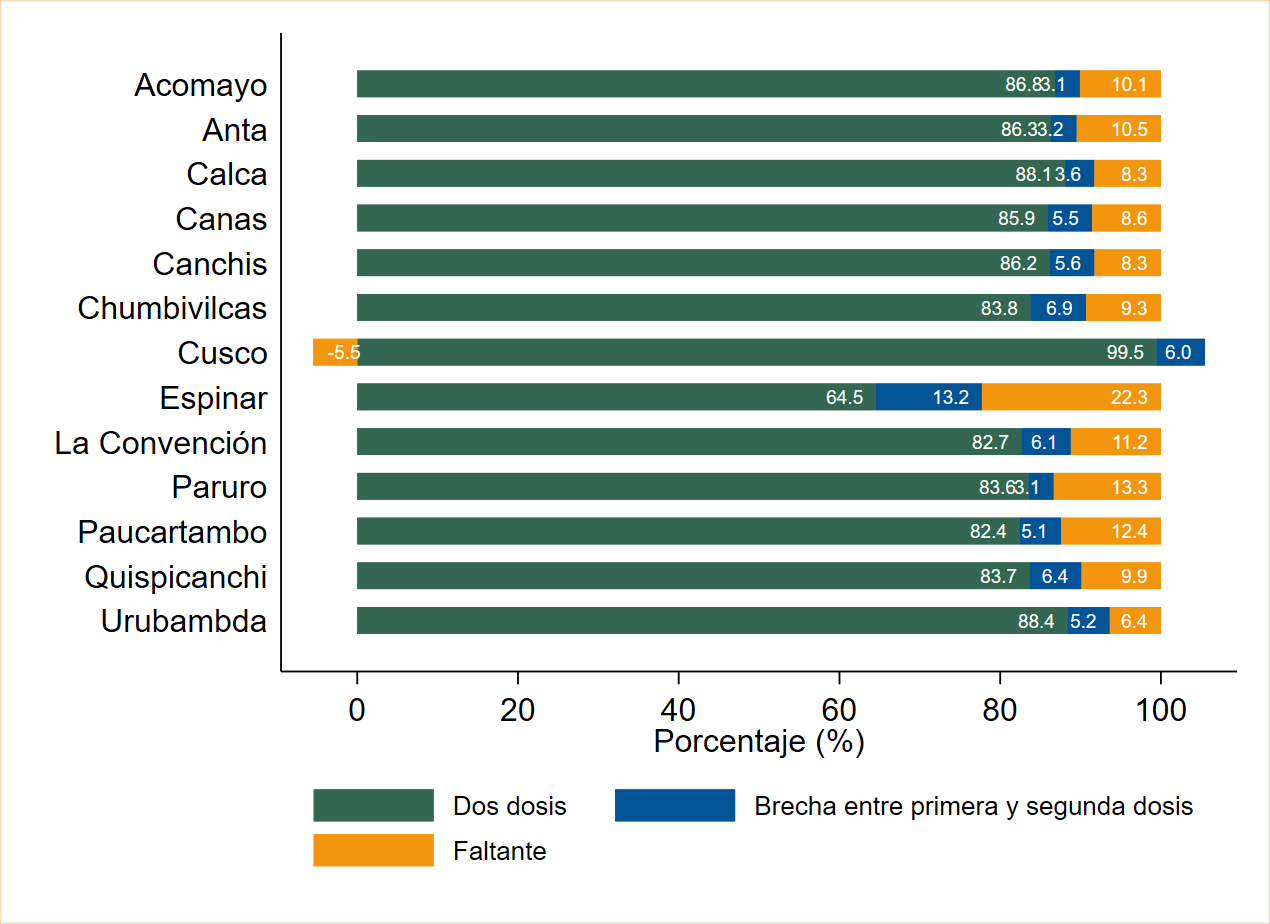
\includegraphics[width=\textwidth]{../figuras/vacunacion_provincial_edad_7}
%	\caption{Más de 80 años}
%	%\label{fig:40 a 49 años}
%\end{subfigure}
%\end{figure}

\clearpage
\subsection*{Análisis de Supervivencia y Vacunas en Hospitalizados con COVID-19 de la Región Cusco}
\noindent Las curvas de sobrevida (Figura \ref{fig:supervivencia_2}) mostraron que los hospitalizados por COVID-19 con tres o dos dosis completas presentan menor probabilidad de muerte, a partir de su ingreso hasta el alta o defunción. Habiendo fallecido con tres dosis el 0.31$\%$, con dos dosis el 5.35$\%$ versus el 89.14$\%$ que no tuvo vacunación. 
Las curvas de sobrevida en hospitalizados por COVID-19 comenzaron a divergir en el 70$\%$ de eventos de muerte en día 18 después del ingreso (long rank test <0,0001).

\begin{figure}[h]
	\caption{Defunciones en vacunados durante la hospitalización en la Región Cusco hasta la SE 07-2022.}\label{fig:supervivencia_2}
	\begin{center}
		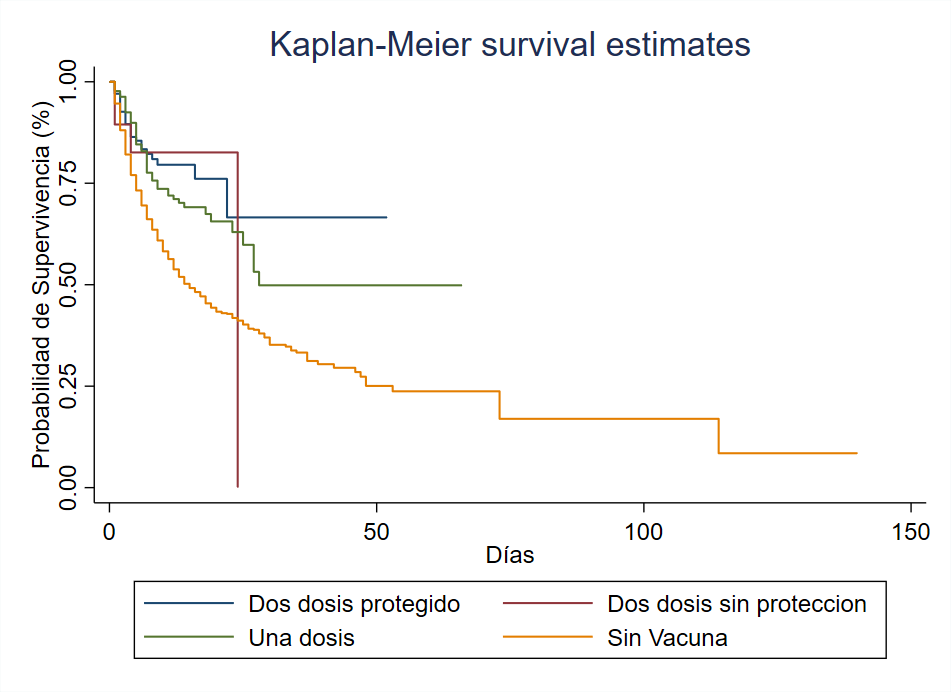
\includegraphics[width=0.90\linewidth]{../figuras/supervivencia_1.png}
	\end{center}
	{\footnotesize {Fuente de datos: SICOVAC, Referencias y contrareferencias.}}
\end{figure}

Las curvas de sobrevida (Figura \ref{fig:supervivencia_2}) mostraron que, conforme al grupo etario de un hospitalizado por COVID-19, se tuvo mayor sobrevida en los grupos de 0 a 17 años, siendo el grupo de mayores de 60 años el que tuvo menor sobrevida durante la hospitalización (long rank test <0,0001).

\begin{figure}[h]
	\caption{Defunciones en vacunados durante la hospitalización conforme al grupo etario, Región Cusco hasta la SE 07-2022. }\label{fig:supervivencia_2}
	\begin{center}
		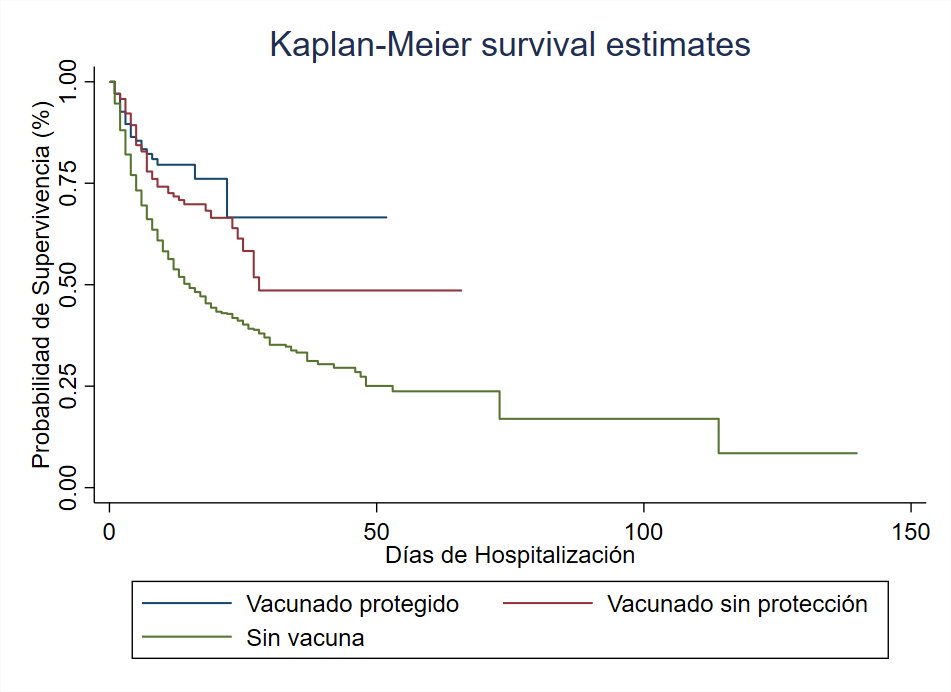
\includegraphics[width=0.90\linewidth]{../figuras/supervivencia_2.png}
	\end{center}
	{\footnotesize {Fuente de datos: SICOVAC, Referencias y contrareferencias}}
\end{figure}

Para la evaluación de muerte relacionada con COVID-19 a partir de la última dosis de vacunación (Figura \ref{fig:supervivencia_4}), se verificó diferencias entre la aplicación de dosis incompleta (1 dosis) versus dosis completas (2 dosis), siendo muy escaso el número de hospitalizados con 3 dosis. Se observó divergencia en la presentación de muerte en el 88.5$\%$ alrededor del día 14 después de la última dosis de vacunación para las personas que presentaron dosis incompletas y completas. (long rank test <0.001)

%\begin{figure}[h]
%	\caption{Defunciones en vacunados durante la hospitalización a partir de la última dosis de vacunación, Región Cusco hasta la SE 07-2022. }\label{fig:supervivencia_4}
%	\begin{center}
%		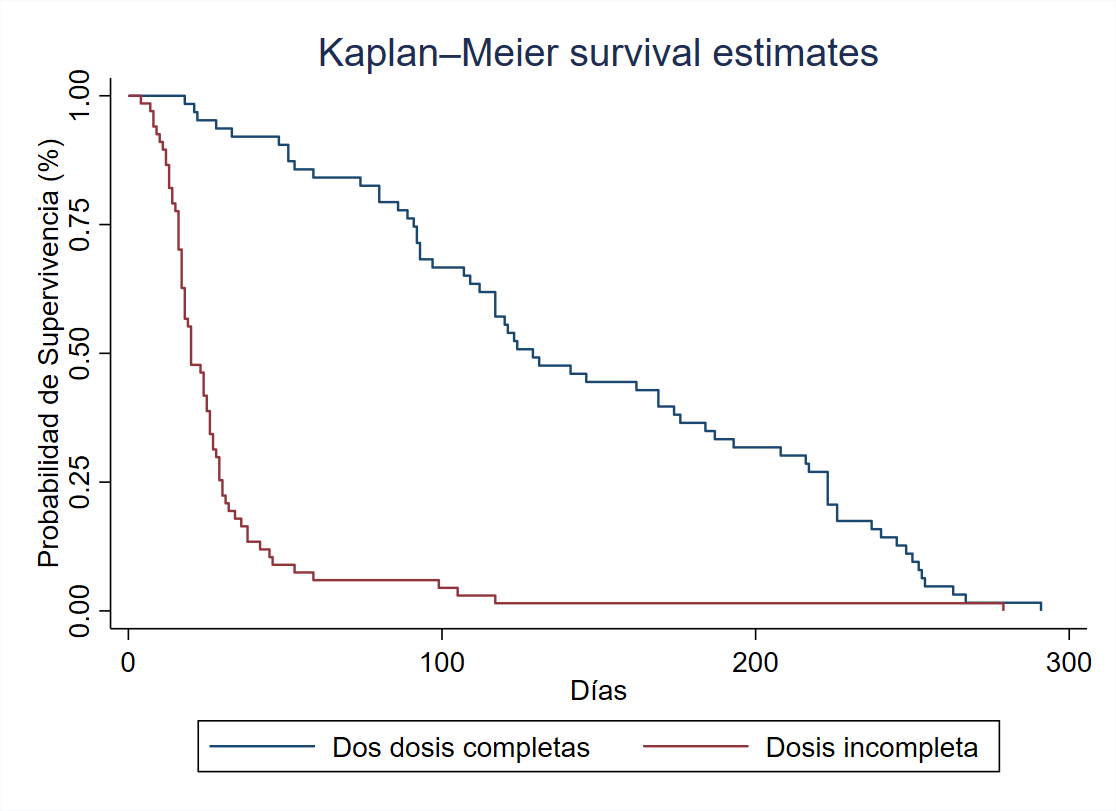
\includegraphics[width=0.90\linewidth]{../figuras/supervivencia_4.png}
%	\end{center}
%	{\footnotesize {Fuente de datos: SICOVAC, Referencias y contrareferencias}}
%\end{figure}


\clearpage
\subsection*{Ocupación de Camas}
\noindent La disponibilidad y ocupación de camas UCI se ve resumida en la Figura \ref{fig:ocupacion_uci}, se evidencia que desde la primera semana del 2022, el porcentaje de ocupación muestra un pendiente en ascenso hasta la SE 06 con el 91$\%$ de camas ocupadas, para la SE 07 el porcentaje de ocupación de camas UCI fue de 88 $\%$. 

\begin{figure}[h]
	\caption{Ocupación de Camas UCI COVID-19 en la Región Cusco hasta la SE 07- 2022.}\label{fig:ocupacion_uci}
	\begin{center}
		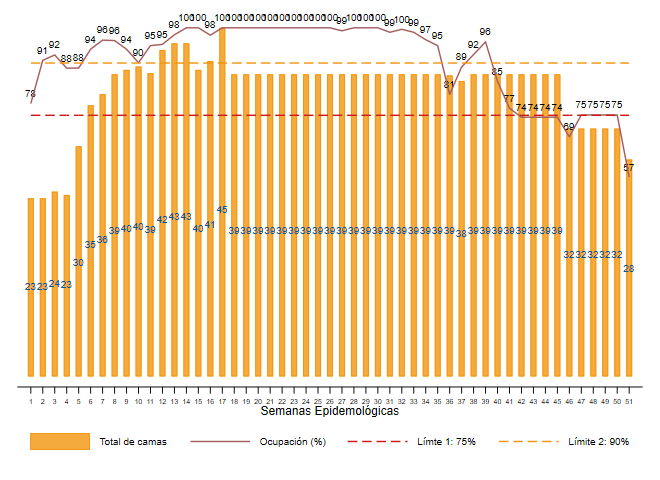
\includegraphics[width=0.95\linewidth]{../figuras/uci.png}
	\end{center}
	{\footnotesize {Fuente de datos: REFERENCIAS Y CONTRAREFERENCIAS.}}
\end{figure}
\cleardoublepage

En la Figura \ref{fig:ocupacion_3_nivel}, se plasma el porcentaje de ocupación y número de camas no-UCI COVID-19 en el nivel Hospitalario III. Se evidencia que tras el inicio de la tercera ola, el porcentaje de ocupación de camas ascendió hasta 54$\%$ en la SE 04, tras lo cual fue descendiento paulatinamente. Para la SE 07 el porcentaje de ocupación fue de 26 $\%$.    
  
\begin{figure}[htpb]
	\caption{Ocupación de Camas no UCI COVID-19 en el nivel III en la Región Cusco hasta la SE 07-2022.}\label{fig:ocupacion_3_nivel}
	\begin{center}
		\includegraphics[width=0.95\linewidth]{../figuras/nivel_3.png}
	\end{center}
	{\footnotesize {Fuente de datos: REFERENCIAS Y CONTRAREFERENCIAS.}}
\end{figure}

\clearpage

En la Figura \ref{fig:ocupacion_2nivel}, se observa el número de camas disponibles y su porcentaje de ocupación en el Nivel II. Hasta la SE 07 el porcentaje de ocupación de camas durante el 2022 se ha mantenido por debajo del 25 $\%$, para la última semana sólo el 14 $\%$ de camas fue ocupado. 

\begin{figure}[h]
	\caption{Disponibilidad y Ocupación de Camas-COVID a Nivel de Hospitales del Nivel II en la Región Cusco hasta la SE 07-2022.}\label{fig:ocupacion_2nivel}
	\begin{center}
		\includegraphics[width=0.95\linewidth]{../figuras/nivel_2.png}
	\end{center}
	{\footnotesize {Fuente de datos: REFERENCIAS Y CONTRAREFERENCIAS.}}
\end{figure}
\clearpage
\begin{landscape}
	
	\subsection*{Evaluación Provincial de la Infección por COVID-19 para el año 2022.} 
	
	\begin{tabular}{@{}lrrrrr@{}}
	\rowcolor[HTML]{ECF4FF} 
	\textbf{Provincias}                   & \multicolumn{1}{l}{\cellcolor[HTML]{ECF4FF}\textbf{población}} & \multicolumn{1}{l}{\cellcolor[HTML]{ECF4FF}\textbf{Pruebas Totales}} & \multicolumn{1}{l}{\cellcolor[HTML]{ECF4FF}\textbf{Funciones}} & \multicolumn{1}{l}{\cellcolor[HTML]{ECF4FF}\textbf{Tasa de letalidad}} & \multicolumn{1}{l}{\cellcolor[HTML]{ECF4FF}\textbf{\begin{tabular}[c]{@{}l@{}}tasa de mortalidad x \\   100.000 hab\end{tabular}}} \\
	\cellcolor[HTML]{FD6864}CANCHIS       & 105,049                                                        & 1,545                                                                & 5                                                              & 0.3\%                                                                  & 4.8                                                                                                                                \\
	\cellcolor[HTML]{FD6864}PAUCARTAMBO   & 52,989                                                         & 301                                                                  & 2                                                              & 0.7\%                                                                  & 3.8                                                                                                                                \\
	\cellcolor[HTML]{FD6864}LA CONVENCION & 185,793                                                        & 2,623                                                                & 7                                                              & 0.3\%                                                                  & 3.8                                                                                                                                \\
	\cellcolor[HTML]{FFFC9E}CUSCO         & 463,656                                                        & 16,911                                                               & 9                                                              & 0.1\%                                                                  & 1.9                                                                                                                                \\
	\cellcolor[HTML]{FFFC9E}ESPINAR       & 71,304                                                         & 479                                                                  & 1                                                              & 0.2\%                                                                  & 1.4                                                                                                                                \\
	\cellcolor[HTML]{FFFC9E}CALCA         & 76,462                                                         & 462                                                                  & 1                                                              & 0.2\%                                                                  & 1.3                                                                                                                                \\
	\cellcolor[HTML]{9AFF99}CHUMBIVILCAS  & 84,925                                                         & 448                                                                  & 1                                                              & 0.2\%                                                                  & 1.2                                                                                                                                \\
	\cellcolor[HTML]{9AFF99}QUISPICANCHI  & 92,566                                                         & 735                                                                  & 1                                                              & 0.1\%                                                                  & 1.1                                                                                                                                \\
	\cellcolor[HTML]{9AFF99}ACOMAYO       & 28,477                                                         & 149                                                                  & 0                                                              & 0.0\%                                                                  & 0.0                                                                                                                                \\
	\cellcolor[HTML]{9AFF99}ANTA          & 57,731                                                         & 480                                                                  & 0                                                              & 0.0\%                                                                  & 0.0                                                                                                                                \\
	\cellcolor[HTML]{9AFF99}CANÁS         & 40,420                                                         & 206                                                                  & 0                                                              & 0.0\%                                                                  & 0.0                                                                                                                                \\
	\cellcolor[HTML]{9AFF99}PARURO        & 31,264                                                         & 132                                                                  & 0                                                              & 0.0\%                                                                  & 0.0                                                                                                                                \\
	\cellcolor[HTML]{9AFF99}URUBAMBÁ      & 66,439                                                         & 900                                                                  & 0                                                              & 0.0\%                                                                  & 0.0                                                                                                                                \\
	& \multicolumn{1}{l}{}                                           & \multicolumn{1}{l}{}                                                 & \multicolumn{1}{l}{}                                           & \multicolumn{1}{l}{}                                                   & \multicolumn{1}{l}{}                                                                                                               \\
	\rowcolor[HTML]{ECF4FF} 
	\textbf{Totales generales}            & \textbf{1,357,075}                                             & \textbf{25,371}                                                      & \textbf{27}                                                    & \textbf{0.11\%}                                                        & \textbf{2.0}                                                                                                                      
\end{tabular}
	
	
	{\footnotesize Fuente de datos: NOTICOVID, SISCOVID, SINADEF. Actualizado a la SE 07-2022.}
	
	\noindent 
	
\end{landscape}
%---------------------------------------------------------------------------
% CAPÍTULO: EVALUACIÓN DE PROVINCIAS
%---------------------------------------------------------------------------

%insertar el cover del capitulo
\includepdf[pages={1}]{../editorial/5.pdf}
\clearpage

	\section*{Evaluación para Provincias Priorizadas}
\addcontentsline{toc}{chapter}{Evaluación para Provincias Priorizadas}
\noindent La Figura \ref{fig:incidencia_provincias} muestra las tasas de incidencia acumulada por provincia desde el 1 de enero hasta el 22 de febrero del 2022, ordenadas de mayor a menor, se evidencia que la mayor tasa de incidencia acumulada es la provincia de Cusco (619,9 casos / 10 000 personas), seguida de la provincia de Canchis (279,9 casos/ 10 000 personas)  y Urubamba (238,9 casos/ 10 000 personas).

\begin{figure}[!htpb]
	\caption{Tasa de Incidencia Acumulada por Provincia en la Región Cusco, hasta el 22 de febrero del 2022*. }\label{fig:incidencia_provincias}
	\begin{center}
		\includegraphics[width=0.60\linewidth]{../figuras/incidencia_provincial_2022.png}
	\end{center}
	{\footnotesize {
	Fuente de datos: SISCOVID, NOTICOVID.(*)Se considera como caso positivo sólo a pacientes con prueba molecular o antigénica positiva}}
\end{figure}

La Figura \ref{fig:mortalidad_ordenada} muestra a las provincias de la región ordenadas de mayor a menor según la tasa de mortalidad acumulada, desde el 1 de enero hasta el 22 de febrero del 2022. La mayor tasa de mortalidad persiste en la provincia de Canchis con 1,9 defunciones / 10 000 personas.   

\begin{figure}[h]
	\caption{Tasa de Mortalidad Acumulada por Provincia en la Región Cusco, hasta la SE 07-2022. }\label{fig:mortalidad_ordenada}
	\begin{center}
		\includegraphics[width=0.60\linewidth]{../figuras/mortalidad_provincial_2022.png}
	\end{center}
	{\footnotesize {Fuente de datos: SISCOVID, NOTICOVID.}}
\end{figure}

La Figura \ref{fig:incidencia_provincial} muestra la tendencia de la incidencia acumulada a través del año 2022. Se evidencia que la tasa de incidencia se presenta en meseta desde la SE 05, luego de presentar un incremento abrupto en las semanas previas. 
%
\begin{figure}[h]
	\caption{Tendencia Provincial de Incidencia acumulada de COVID-19 hasta la SE 07-2022. }\label{fig:incidencia_provincial}
	\begin{center}
		\includegraphics[width=0.60\linewidth]{../figuras/incidencia_provincial_acumulada_2022.pdf}
	\end{center}
	{\footnotesize {Fuente de datos: SINADEF.}}
\end{figure}

\clearpage
	
\section*{Evaluación Provincial de 5 Indicadores}
		\noindent El objetivo de estas figuras es comparar a cada provincia consigo misma de acuerdo a su historia  en la primera ola (en el año 2020). Se evaluaron los siguientes indicadores: incidencia (tomando en cuenta pruebas moleculares y antigénicas), tasa de mortalidad, tasa de positividad por prueba molecular, tasa de positividad por prueba antigénica, y exceso de defunciones para cada provincia.
		
		\subsection*{Provincia de Acomayo}
		\noindent La Figura \ref{fig:inc_mort_acomayo} se evidencia un ascenso de la tasa de incidencia a partir de la SE 01 del año 2022 hasta la SE 05 donde comienza su descenso. Con respecto a la tasa de mortalidad, se reportaron muertes durante la SE 05 y SE 06. 
		\noindent La figura Figura \ref{fig:positividad_acomayo} muestra la tendencia al descenso de la tasa de positividad de ambas pruebas. 
		
		 En la Figura \ref{fig:exceso_acomayo} se muestra que hay exceso de 3 defunciones respecto al año 2019.
		
		\begin{figure}[h]
			\caption{Tasa de Incidencia y Mortalidad Comparativa en la Provincia de Acomayo hasta la SE 07-2022.}\label{fig:inc_mort_acomayo}
			\begin{center}
				\includegraphics[width=0.70\linewidth]{../figuras/incidencia_mortalidad_20_21_1.png}
			\end{center}
			{\footnotesize {Fuente de datos: NOTICOVID, SISCOVID, SINADEF.}}
		\end{figure}
		
		\begin{figure}[h]
			\caption{Tasa de Positividad de Prueba Molecular y Antigénica Comparativa en la Provincia de Acomayo hasta la SE 07-2022. }\label{fig:positividad_acomayo}
			\begin{center}
				\includegraphics[width=0.7\linewidth]{../figuras/positividad_20_21_1.png}
			\end{center}
			{\footnotesize {Fuente de datos: NOTICOVID, SISCOVID.}}
		\end{figure}
		
		\begin{figure}[h]
			\caption{Exceso de Defunciones Comparativo en la Provincia de Acomayo hasta la SE 07-2022.}\label{fig:exceso_acomayo}
			\begin{center}
				\includegraphics[width=0.7\linewidth]{../figuras/exceso_1.pdf}
			\end{center}
			{\footnotesize {Fuente de datos: SINADEF.}}
		\end{figure}
		
		% Anta
		\clearpage
		
		\subsection*{Provincia de Anta}
		\noindent La Figura \ref{fig:inc_mort_anta} se observa la tendencia al descenso de la tasa de incidencia a partir de la SE 03. Con respecto a la tasa de mortalidad se reportaron muertes en la SE 04 y SE 06.
		\noindent La Figura
		\ref{fig:positividad_anta} la disminución en la última semana de la tasa de positividad de pruebas moleculares y antigénicas. 
		
		En la Figura \ref{fig:exceso_anta} se muestra que hay exceso de 4 defunciones respecto al año 2019.
		
		\begin{figure}[h]
			\caption{Tasa de Incidencia y Mortalidad Comparativa en la Provincia de Anta hasta la SE 07-2022.}\label{fig:inc_mort_anta}
			\begin{center}
				\includegraphics[width=0.85\linewidth]{../figuras/incidencia_mortalidad_20_21_2.png}
			\end{center}
			{\footnotesize {Fuente de datos: NOTICOVID, SISCOVID, SINADEF.}}
		\end{figure}
		
		\begin{figure}[h]
			\caption{Tasa de Positividad de Prueba Molecular y Antigénica Comparativa en la Provincia de Anta hasta la SE 07-2022.}\label{fig:positividad_anta}
			\begin{center}
				\includegraphics[width=0.7\linewidth]{../figuras/positividad_20_21_2.png}
			\end{center}
			{\footnotesize {Fuente de datos: NOTICOVID, SISCOVID.}}
		\end{figure}
		
		\begin{figure}[h]
			\caption{Exceso de Defunciones Comparativo en la Provincia de Anta hasta la SE 07-2022.}\label{fig:exceso_anta}
			\begin{center}
				\includegraphics[width=0.7\linewidth]{../figuras/exceso_2.pdf}
			\end{center}
			{\footnotesize {Fuente de datos: SINADEF.}}
		\end{figure}
		
		% Canas
		\clearpage
		
		\subsection*{Provincia de Canas}
		\noindent La Figura \ref{fig:inc_mort_canas} se evidencia un descenso de la tasa de incidencia a partir de la SE 03 del año 2022, mientras que se reportó un incremento de muertes en la SE 06. 
		\noindent La Figura \ref{fig:positividad_canas} muestra una tendencia al descenso de la tasa de positividad de pruebas antigénicas y moleculares. 
		
		La Figura \ref{fig:exceso_canas} muestra que hay exceso de 4 defunciones respecto al año 2019.
		
		\begin{figure}[h]
			\caption{Tasa de Incidencia y Mortalidad Comparativa en la Provincia de Canas hasta la SE 07-2022.}\label{fig:inc_mort_canas}
			\begin{center}
				\includegraphics[width=0.85\linewidth]{../figuras/incidencia_mortalidad_20_21_3.png}
			\end{center}
			{\footnotesize {Fuente de datos: NOTICOVID, SISCOVID, SINADEF.}}
		\end{figure}
		
		\begin{figure}[h]
			\caption{Tasa de Positividad de Prueba Molecular y Antigénica Comparativa en la Provincia de Canas hasta la SE 07-2022.}\label{fig:positividad_canas}
			\begin{center}
				\includegraphics[width=0.7\linewidth]{../figuras/positividad_20_21_3.png}
			\end{center}
			{\footnotesize {Fuente de datos: NOTICOVID, SISCOVID.}}
		\end{figure}
		
		\begin{figure}[h]
			\caption{Exceso de Defunciones Comparativo en la Provincia de Canas hasta la SE 07-2022.}\label{fig:exceso_canas}
			\begin{center}
				\includegraphics[width=0.7\linewidth]{../figuras/exceso_3.pdf}
			\end{center}
			{\footnotesize {Fuente de datos: SINADEF.}}
		\end{figure}
		
		% Calca
		\clearpage
		
		\subsection*{Provincia de Calca}
		\noindent Las figuras de abajo (Figura \ref{fig:inc_mort_calca}, \ref{fig:positividad_calca}) muestran el comportamiento de la tasa de incidencia, mortalidad y  positividad. Con respecto a la tasa de incidencia se evidencia su tendencia al descenso desde la SE 05, mientras que la tasa de mortalidad ha incrementado en la SE 07.  
		
		En la Figura \ref{fig:exceso_calca} se muestra que hay exceso de 4 defunciones respecto al año 2019.
		
		\begin{figure}[h]
			\caption{Tasa de Incidencia y Mortalidad Comparativa en la Provincia de Calca hasta la SE 07-2022.}\label{fig:inc_mort_calca}
			\begin{center}
				\includegraphics[width=0.85\linewidth]{../figuras/incidencia_mortalidad_20_21_4.pdf}
			\end{center}
			{\footnotesize {Fuente de datos: NOTICOVID, SISCOVID, SINADEF.}}
		\end{figure}
		
		\begin{figure}[h]
			\caption{Tasa de Positividad de Prueba Molecular y Antigénica Comparativa en la Provincia de Calca hasta la SE 07-2022.}\label{fig:positividad_calca}
			\begin{center}
				\includegraphics[width=0.7\linewidth]{../figuras/positividad_20_21_4.pdf}
			\end{center}
			{\footnotesize {Fuente de datos: NOTICOVID, SISCOVID.}}
		\end{figure}
		
		\begin{figure}[h]
			\caption{Exceso de Defunciones Comparativo en la Provincia de Calca hasta la SE 07-2022.}\label{fig:exceso_calca}
			\begin{center}
				\includegraphics[width=0.7\linewidth]{../figuras/exceso_4.pdf}
			\end{center}
			{\footnotesize {Fuente de datos: SINADEF.}}
		\end{figure}
		
		% Canchis
		\clearpage
		
		\subsection*{Provincia de Canchis}
		\noindent La Figura \ref{fig:inc_mort_canchis} muestra la tendencia al descenso de la tasa de incidencia a partir de la SE 05. Con respecto a la tasa de mortalidad se reportaron muertes en la SE 03 y SE 06.    
		\noindent La Figura \ref{fig:positividad_canchis} muestra el descenso de las tasas de positividad de ambas pruebas desde la SE 05.
		
		En la Figura \ref{fig:exceso_canchis} se muestra que hay exceso de menos 02 defunciones (exceso negativo) respecto al año 2019.
		
		\begin{figure}[h]
			\caption{Tasa de Incidencia y Mortalidad Comparativa en la Provincia de Canchis hasta la SE 07-2022.}\label{fig:inc_mort_canchis}
			\begin{center}
				\includegraphics[width=0.85\linewidth]{../figuras/incidencia_mortalidad_20_21_5.png}
			\end{center}
			{\footnotesize {Fuente de datos: NOTICOVID, SISCOVID, SINADEF.}}
		\end{figure}
		
		\begin{figure}[h]
			\caption{Tasa de Positividad de Prueba Molecular y Antigénica Comparativa en la Provincia de Canchis hasta la SE 07-2022.}\label{fig:positividad_canchis}
			\begin{center}
				\includegraphics[width=0.7\linewidth]{../figuras/positividad_20_21_5.png}
			\end{center}
			{\footnotesize {Fuente de datos: NOTICOVID, SISCOVID.}}
		\end{figure}
		
		\begin{figure}[h]
			\caption{Exceso de Defunciones Comparativo en la Provincia de Canchis hasta la SE 07-2022.}\label{fig:exceso_canchis}
			\begin{center}
				\includegraphics[width=0.7\linewidth]{../figuras/exceso_5.pdf}
			\end{center}
			{\footnotesize {Fuente de datos: SINADEF.}}
		\end{figure}
		
		\clearpage
		
		% Chumbivilcas
		\subsection*{Provincia de Chumbivilcas}
		\noindent La Figura \ref{fig:inc_mort_chumbivilcas} se evidencia un descenso en la tasa de mortalidad desde la SE 03. Sin embargo, la tasa de mortalidad muestra una tendencia al ascenso desde la SE 05.   
		\noindent La Figura \ref{fig:positividad_chumbivilcas} muestra una tendencia al descenso de la tasa de positividad de pruebas antigénicas desde la SE 03, mientras que la positividad de pruebas moleculares se ha mantenido variable. 
		
		En la Figura \ref{fig:exceso_chumbivilcas} se muestra que hay exceso de 3 defunciones respecto al año 2019.
		
		\begin{figure}[h]
			\caption{Tasa de Incidencia y Mortalidad Comparativa en la Provincia de Chumbivilcas hasta la SE 07-2022.}\label{fig:inc_mort_chumbivilcas}
			\begin{center}
				\includegraphics[width=0.85\linewidth]{../figuras/incidencia_mortalidad_20_21_6.png}
			\end{center}
			{\footnotesize {Fuente de datos: NOTICOVID, SISCOVID, SINADEF.}}
		\end{figure}
		
		\begin{figure}[h]
			\caption{Tasa de Positividad de Prueba Molecular y Antigénica Comparativa en la Provincia de Chumbivilcas 2020 hasta la SE 07-2022.}\label{fig:positividad_chumbivilcas}
			\begin{center}
				\includegraphics[width=0.7\linewidth]{../figuras/positividad_20_21_6.png}
			\end{center}
			{\footnotesize {Fuente de datos: NOTICOVID, SISCOVID.}}
		\end{figure}
		
		\begin{figure}[h]
			\caption{Exceso de Defunciones Comparativo en la Provincia de Chumbivilcas hasta la SE 07-2022.}\label{fig:exceso_chumbivilcas}
			\begin{center}
				\includegraphics[width=0.7\linewidth]{../figuras/exceso_6.pdf}
			\end{center}
			{\footnotesize {Fuente de datos: SINADEF.}}
		\end{figure}
		
		% Cusco
		\clearpage
		
		\subsection*{Provincia de Cusco}
		\noindent La Figura \ref{fig:inc_mort_cusco} se evidencia un descenso marcado de la tasa de incidencia desde la SE 03, mientras que la tasa de mortalidad muestra un discreto ascenso en la SE 07.   
		\noindent La  Figura \ref{fig:positividad_cusco} muestra el mismo comportamiento para la tasa de positividad de ambas pruebas a partir de la SE 04 del 2022. 
	
	En la Figura \ref{fig:exceso_cusco} se muestra que hay exceso de 14 defunciones respecto al año 2019.
		
		\begin{figure}[h]
			\caption{Tasa de Incidencia y Mortalidad Comparativa en la Provincia de Cusco hasta la SE 07-2022.}\label{fig:inc_mort_cusco}
			\begin{center}
				\includegraphics[width=0.85\linewidth]{../figuras/incidencia_mortalidad_20_21_7.png}
			\end{center}
			{\footnotesize {Fuente de datos: NOTICOVID, SISCOVID, SINADEF.}}
		\end{figure}
		
		\begin{figure}[h]
			\caption{Tasa de Positividad de Prueba Molecular y Antigénica Comparativa en la Provincia de Cusco hasta la SE 07-2022.}\label{fig:positividad_cusco}
			\begin{center}
				\includegraphics[width=0.7\linewidth]{../figuras/positividad_20_21_7.png}
			\end{center}
			{\footnotesize {Fuente de datos: NOTICOVID, SISCOVID.}}
		\end{figure}
		
		\begin{figure}[h]
			\caption{Exceso de Defunciones Comparativo en la Provincia de Cusco hasta la SE 07-2022.}\label{fig:exceso_cusco}
			\begin{center}
				\includegraphics[width=0.7\linewidth]{../figuras/exceso_7.pdf}
			\end{center}
			{\footnotesize {Fuente de datos: SINADEF.}}
		\end{figure}
		
		% Espinar
		\clearpage
		
		\subsection*{Provincia de Espinar}
		\noindent Las figuras de abajo (Figura \ref{fig:inc_mort_espinar}, \ref{fig:positividad_espinar}) muestran el comportamiento de la tasa de incidencia, mortalidad y positividad. Se evidencia la tendencia al descenso de la tasa de incidencia desde la SE 03, mientras que la tasa de mortalidad presenta una tendencia discreta al ascenso en la SE 07.  
		
		En la Figura \ref{fig:exceso_espinar} se muestra que hay exceso de 5 defunciones respecto al año 2019.
		
		\begin{figure}[h]
			\caption{Tasa de Incidencia y Mortalidad Comparativa en la Provincia de Espinar hasta la SE 07-2022.}\label{fig:inc_mort_espinar}
			\begin{center}
				\includegraphics[width=0.85\linewidth]{../figuras/incidencia_mortalidad_20_21_8.png}
			\end{center}
			{\footnotesize {Fuente de datos: NOTICOVID, SISCOVID, SINADEF.}}
		\end{figure}
		
		\begin{figure}[h]
			\caption{Tasa de Positividad de Prueba Molecular y Antigénica Comparativa en la Provincia de Espinar hasta la SE 07-2022.}\label{fig:positividad_espinar}
			\begin{center}
				\includegraphics[width=0.7\linewidth]{../figuras/positividad_20_21_8.png}
			\end{center}
			{\footnotesize {Fuente de datos: NOTICOVID, SISCOVID.}}
		\end{figure}
		
		\begin{figure}[h]
			\caption{Exceso de Defunciones Comparativo en la Provincia de Espinar hasta la SE 07-2022.}\label{fig:exceso_espinar}
			\begin{center}
				\includegraphics[width=0.7\linewidth]{../figuras/exceso_8.pdf}
			\end{center}
			{\footnotesize {Fuente de datos: SINADEF.}}
		\end{figure}
		
		% La Convención
		\clearpage
		
		\subsection*{Provincia de La Convención}
		\noindent Las figuras inferiores (Figura \ref{fig:inc_mort_laconv}, \ref{fig:positividad_laconv}) muestran el comportamiento de la tasa de incidencia y mortalidad, con respecto a la tasa de incidencia se muestra una tendencia al descenso desde la SE 03. Mientras que la tasa de mortalidad se ha mantenido en ascenso discreto desde la SE 02. 
	
	En la Figura \ref{fig:exceso_laconv}  muestra que hay exceso de 2 defunciones respecto al año 2019.     
	
		\begin{figure}[h]
			\caption{Tasa de Incidencia y Mortalidad Comparativa en la Provincia de La Convención hasta la SE 07-2022.}\label{fig:inc_mort_laconv}
			\begin{center}
				\includegraphics[width=0.85\linewidth]{../figuras/incidencia_mortalidad_20_21_9.png}
			\end{center}
			{\footnotesize {Fuente de datos: NOTICOVID, SISCOVID, SINADEF.}}
		\end{figure}
		
		\begin{figure}[h]
			\caption{Tasa de Positividad de Prueba Molecular y Antigénica Comparativa en la Provincia de La Convención hasta la SE 07-2022.}\label{fig:positividad_laconv}
			\begin{center}
				\includegraphics[width=0.7\linewidth]{../figuras/positividad_20_21_9.png}
			\end{center}
			{\footnotesize {Fuente de datos: NOTICOVID, SISCOVID.}}
		\end{figure}
		
		\begin{figure}[h]
			\caption{Exceso de Defunciones Comparativo en la Provincia de La Convención hasta la SE 07-2022.}\label{fig:exceso_laconv}
			\begin{center}
				\includegraphics[width=0.7\linewidth]{../figuras/exceso_9.pdf}
			\end{center}
			{\footnotesize {Fuente de datos: SINADEF.}}
		\end{figure}
		
		% Paruro
		\clearpage
		
		\subsection*{Provincia de Paruro}
		\noindent Las figuras de abajo (Figura \ref{fig:inc_mort_paruro}, \ref{fig:positividad_paruro}) muestran el comportamiento de la tasa de incidencia, mortalidad y positividad. Para la SE 07 la tasa de incidencia muestra una pendiente al ascenso al igual que la tasa de mortalidad.
	 
	 En la Figura \ref{fig:exceso_paruro} muestra que no hubieron exceso de muertes. 
		
		\begin{figure}[h]
			\caption{Tasa de Incidencia y Mortalidad Comparativa en la Provincia de Paruro, hasta la SE 07-2022.}\label{fig:inc_mort_paruro}
			\begin{center}
				\includegraphics[width=0.85\linewidth]{../figuras/incidencia_mortalidad_20_21_10.png}
			\end{center}
			{\footnotesize {Fuente de datos: NOTICOVID, SISCOVID, SINADEF.}} 
		\end{figure}
		
		\begin{figure}[h]
			\caption{Tasa de Positividad de Prueba Molecular y Antigénica Comparativa en la Provincia de Paruro hasta la SE 07-2022.}\label{fig:positividad_paruro}
			\begin{center}
				\includegraphics[width=0.7\linewidth]{../figuras/positividad_20_21_10.png}
			\end{center}
			{\footnotesize {Fuente de datos: NOTICOVID, SISCOVID.}}
		\end{figure}
		
		\begin{figure}[h]
			\caption{Exceso de Defunciones Comparativo en la Provincia de Paruro hasta la SE 07-2022.}\label{fig:exceso_paruro}
			\begin{center}
				\includegraphics[width=0.7\linewidth]{../figuras/exceso_10.pdf}
			\end{center}
			{\footnotesize {Fuente de datos: SINADEF.}}
		\end{figure}
		
		
		% Paucartambo
		\clearpage
		
		\subsection*{Provincia de Paucartambo}
		\noindent Las figuras de abajo (Figura \ref{fig:inc_mort_paucartam}, \ref{fig:positividad_paucartam}) muestran el comportamiento de la tasa de incidencia, mortalidad y positividad. Se evidencia la tendencia al descenso de la tasa de incidencia desde la SE 05 al igual que la tasa de mortalidad.   
	En la Figura \ref{fig:exceso_paucartam} se muestra que hay exceso de 1 defunción respecto al año 2021.  
		
		\begin{figure}[h]
			\caption{Tasa de Incidencia y Mortalidad Comparativa en la Provincia de Paucartambo hasta la SE 07-2022.}\label{fig:inc_mort_paucartam}
			\begin{center}
				\includegraphics[width=0.85\linewidth]{../figuras/incidencia_mortalidad_20_21_11.png}
			\end{center}
			{\footnotesize {Fuente de datos: NOTICOVID, SISCOVID, SINADEF.}}
		\end{figure}
		
		\begin{figure}[h]
			\caption{Tasa de Positividad de Prueba Molecular y Antigénica Comparativa en la Provincia de Paucartambo hasta la SE 07-2022.}\label{fig:positividad_paucartam}
			\begin{center}
				\includegraphics[width=0.7\linewidth]{../figuras/positividad_20_21_11.png}
			\end{center}
			{\footnotesize {Fuente de datos: NOTICOVID, SISCOVID.}}
		\end{figure}
		
		\begin{figure}[h]
			\caption{Exceso de Defunciones Comparativo en la Provincia de Paucartambo hasta la SE 07-2022.}\label{fig:exceso_paucartam}
			\begin{center}
				\includegraphics[width=0.7\linewidth]{../figuras/exceso_11.pdf}
			\end{center}
			{\footnotesize {Fuente de datos: SINADEF.}}
		\end{figure}
		
		% Quispicanchi
		\clearpage
		
		\subsection*{Provincia de Quispicanchi}
		\noindent Las figuras de abajo (Figura \ref{fig:inc_mort_quisp}, \ref{fig:positividad_quisp}) muestran el comportamiento de la tasa de incidencia, mortalidad y positividad. La tasa de incidencia muestra una tendencia al descenso desde la SE 03, con respecto a la tasa de mortalidad se reportó un aumento de casos para la SE 04.      
		
	En la Figura \ref{fig:exceso_quisp} se muestra que hay exceso de 1 defunción respectos al año 2019.
		
		\begin{figure}[h]
			\caption{Tasa de Incidencia y Mortalidad Comparativa en la Provincia de Quispicanchi hasta la SE 07-2022.}\label{fig:inc_mort_quisp}
			\begin{center}
				\includegraphics[width=0.85\linewidth]{../figuras/incidencia_mortalidad_20_21_12.png}
			\end{center}
			{\footnotesize {Fuente de datos: NOTICOVID, SISCOVID, SINADEF.}}
		\end{figure}
		
		\begin{figure}[h]
			\caption{Tasa de Positividad de Prueba Molecular y Antigénica Comparativa en la Provincia de Quispicanchi hasta la SE 07-2022.}\label{fig:positividad_quisp}
			\begin{center}
				\includegraphics[width=0.7\linewidth]{../figuras/positividad_20_21_12.png}
			\end{center}
			{\footnotesize {Fuente de datos: NOTICOVID, SISCOVID.}}
		\end{figure}
		
		\begin{figure}[h]
			\caption{Exceso de Defunciones Comparativo en la Provincia de Quispicanchis hasta la SE 07-2022.}\label{fig:exceso_quisp}
			\begin{center}
				\includegraphics[width=0.7\linewidth]{../figuras/exceso_12.pdf}
			\end{center}
			{\footnotesize {Fuente de datos: SINADEF.}}
		\end{figure}
		
		% Urubamba
		\clearpage
		
		\subsection*{Provincia de Urubamba}
		\noindent Las figuras de abajo (Figura \ref{fig:inc_urub}, \ref{fig:positividad_urub}) muestran el comportamiento de la tasa de incidencia, mortalidad y positividad. Con respecto a la tasa de incidencia se evidencia un descenso de la misma desde la SE 03. 
	
		En la Figura \ref{fig:exceso_urub} se muestra que hay exceso de menos 1 defunción (exceso negativo) respecto al año 2019.
		
		\begin{figure}[h]
			\caption{Tasa de Incidencia y Mortalidad Comparativa en la Provincia de Urubamba hasta la SE 07-2022.}\label{fig:inc_urub}
			\begin{center}
				\includegraphics[width=0.85\linewidth]{../figuras/incidencia_mortalidad_20_21_13.png}
			\end{center}
			{\footnotesize {Fuente de datos: NOTICOVID, SISCOVID, SINADEF.}}
		\end{figure}
		
		\begin{figure}[h]
			\caption{Tasa de Positividad de Prueba Molecular y Antigénica Comparativa en la Provincia de Urubamba hasta la SE 07-2022.}\label{fig:positividad_urub}
			\begin{center}
				\includegraphics[width=0.7\linewidth]{../figuras/positividad_20_21_13.png}
			\end{center}
			{\footnotesize {Fuente de datos: NOTICOVID, SISCOVID.}}
		\end{figure}
		
		\begin{figure}[h]
			\caption{Exceso de Defunciones Comparativo en la Provincia de Urubamba hasta la SE 07-2022.}\label{fig:exceso_urub}
			\begin{center}
				\includegraphics[width=0.7\linewidth]{../figuras/exceso_13.pdf}
			\end{center}
			{\footnotesize {Fuente de datos: SINADEF.}}
		\end{figure}
		
		\clearpage
%---------------------------------------------------------------------------
		% CAPÍTULO: VARIANTES DE COVID-19
		%---------------------------------------------------------------------------
		%insertar el cover del capitulo
		\includepdf[pages={1}]{../editorial/6.pdf}
		\clearpage
		
		\section* {Variantes de COVID-19 en la Región Cusco}
		\addcontentsline{toc}{chapter}{Variantes de COVID-19}
		\noindent La aparición de la variante ómicron ha generado la tercera ola de COVID-19 en el Perú debido a su gran transmisibilidad. En la Figura \ref{fig:variantes} se observa que en la región Cusco, la variante ómicron (100$\%$) ha desplazado a las demás variantes en el secuenciamiento genético semanal durante el mes de febrero. 
		Hasta el 22 de febrero del 2022 se secuenciaron 795 muestras a nivel de la región de Cusco	encontrándose las variantes beta (B.1.1.348), gamma (P.1, P.1.7), lambda (C.37), delta (B.1617.2), mu y ómicron (BA.1.1). 
		La vigilancia genómica es realizada en colaboración con 4 instituciones externas a GERESA-Cusco.
						
		\begin{figure}[h]
			\caption{Prevalencia de las variantes de SARS Cov-2 aisladas en la región de Cusco, hasta Febrero-2022. }\label{fig:variantes}
			\begin{center}
				\includegraphics[width=0.85\linewidth]{../figuras/variantes.pdf}
			\end{center}
			{\footnotesize {Fuente de datos: INS-NETLAB, UPCH, UNSAAC}}
		\end{figure}
		
	Asimismo, la Figura \ref{fig:mapa_variantes} muestra las variantes de COVID-19 aisladas por zonas. Se evidencia una mayor distribución de la variante Ómicron en la región a comparación del boletín previo, se espera que este comportamiento persista en el tiempo.  
	
			\begin{figure}[h]
				\caption{Distribución provincial de las variantes de SARS-CoV-2 aisladas en la Región Cusco hasta la SE 07-2022.}
				\label{fig:mapa_variantes}
				\centering
				\begin{subfigure}[b]{0.40\textwidth}
					\centering
					\includegraphics[width=\textwidth]{../figuras/variantes_provincial_lambda.pdf}
					\caption{Variante Lambda}
					%\label{fig:}
				\end{subfigure}
				\hfill
				\begin{subfigure}[b]{0.40\textwidth}
					\centering
					\includegraphics[width=\textwidth]{../figuras/variantes_provincial_gamma.pdf}
					\caption{Variante Gamma}
					%\label{fig:70 a 79 años}
				\end{subfigure}
							
				\begin{subfigure}[b]{0.40\textwidth}
					\centering
					\includegraphics[width=\textwidth]{../figuras/variantes_provincial_delta.pdf}
					\caption{Variante Delta}
					%\label{fig:60 a 69 años}
				\end{subfigure}
			\vspace{0.5mm}
			\hspace{25mm}
			\begin{subfigure}[b]{0.40\textwidth}
				\centering
				\includegraphics[width=\textwidth]{../figuras/variantes_provincial_omicron.png}
				\caption{Variante Ómicron}
				%\label{fig:60 a 69 años}
			\end{subfigure}
			\end{figure}

\clearpage
%---------------------------------------------------------------------------
% CAPÍTULO: DEFUNCIONES CERO
%-------------------------------------------

%insertar el cover del capitulo
\includepdf[pages={1}]{../editorial/7.pdf}
\clearpage
	\section*{Semanas con Cero Defunciones por COVID-19 por Semana a Nivel Provincial}\addcontentsline{toc}{chapter}{Defunciones Cero}
	
\noindent En la tabla inferior se muestra las provincias con cero defunciones reportadas (casillas en amarillo) por cada semana epidemiológica. El reporte de defunciones incrementó  en el mes de enero y febrero, sin embargo no sobrepasaron al reporte de la primera y segunda ola. En las últimas tres semanas doce de las trece provincias reportaron muertes en su territorio, siendo Paucartambo la única provincia que no reportó muertes en ese periodo, asimismo tras 8 semanas sin defunciones notificadas la provincia de Acomayo reportó su primera muerte en la SE 08.    
	\begin{table}[h]		\caption{Defunciones Cero por COVID-19 a nivel Provincial hasta la SE 08-2022.}
		\resizebox{\textwidth}{!}{%
			\begin{tabular}{lccccccccc}
	\textbf{}              	  
	& \multicolumn{1}{l}{}                        
	& \multicolumn{1}{l}{}      
	& \multicolumn{1}{l}{}                         
	& \multicolumn{1}{l}{}                         
	& \multicolumn{1}{l}{}                         
	& \multicolumn{1}{l}{}                        
	& \multicolumn{1}{l}{}                         
	& \multicolumn{1}{l}{} \\                   
	\textbf{}                                                                 				
	&\textbf{SE-31} 							
	&\textbf{SE-32}						
	&\textbf{SE-33}								
	&\textbf{SE-34}					
	&\textbf{SE-35}								
	&\textbf{SE-36}
	&\textbf{SE-37}
	&\textbf{SE-38}\\							
	\textbf{}              	  																
	&\textbf{31jul-06ago}						
	&\textbf{07ago-13ago}						
	&\textbf{14ago-20ago}						
	&\textbf{21ago-27ago}						
	&\textbf{28ago-03sep}
	&\textbf{04sep-10sep}
	&\textbf{11sep-17sep} 
	&\textbf{18sep-24sep} \\
	\textbf{Acomayo}                        												
	&\cellcolor[HTML]{FCC46C}
	&\cellcolor[HTML]{FCC46C}					
	&\cellcolor[HTML]{FCC46C}
	&\cellcolor[HTML]{FCC46C}					
	&\cellcolor[HTML]{FCC46C}
	&\cellcolor[HTML]{FCC46C} 
	&\cellcolor[HTML]{FCC46C}
	&\cellcolor[HTML]{FCC46C}\\
	\textbf{Anta}                                                  				
	&1											
	&\cellcolor[HTML]{FCC46C}					
	&\cellcolor[HTML]{FCC46C}					
	&\cellcolor[HTML]{FCC46C}					
	&\cellcolor[HTML]{FCC46C}
	&\cellcolor[HTML]{FCC46C}	
	&\cellcolor[HTML]{FCC46C}
	&\cellcolor[HTML]{FCC46C}\\					
	\textbf{Calca}      				       									
	&\cellcolor[HTML]{FCC46C}					
	&1											
	&\cellcolor[HTML]{FCC46C}					
	&1											
	&\cellcolor[HTML]{FCC46C}
	&1
	&1
	&\cellcolor[HTML]{FCC46C}\\          			
	\textbf{Canas}                              									
	&\cellcolor[HTML]{FCC46C}
	&1											
	&1
	&\cellcolor[HTML]{FCC46C}					
	&\cellcolor[HTML]{FCC46C}
	&\cellcolor[HTML]{FCC46C}	
	&\cellcolor[HTML]{FCC46C}
	&\cellcolor[HTML]{FCC46C}\\	
	\textbf{Canchis}    						
	&1			
	&\cellcolor[HTML]{FCC46C}					
	&\cellcolor[HTML]{FCC46C}			
	&\cellcolor[HTML]{FCC46C}					
	&1
	&1
	&\cellcolor[HTML]{FCC46C}
	&\cellcolor[HTML]{FCC46C}\\											
	\textbf{Chumbivilcas}                      									
	&\cellcolor[HTML]{FCC46C}
	&\cellcolor[HTML]{FCC46C}					
	&\cellcolor[HTML]{FCC46C}
	&\cellcolor[HTML]{FCC46C}					
	&1
	&\cellcolor[HTML]{FCC46C}
	&1
	&1\\
	\textbf{Cusco}      															
	&2		
	&3											
	&2
	&4											
	&1
	&1
	&\cellcolor[HTML]{FCC46C}
	&\cellcolor[HTML]{FCC46C}\\								
	\textbf{Espinar}       					             							
	&\cellcolor[HTML]{FCC46C}					
	&\cellcolor[HTML]{FCC46C}
	&\cellcolor[HTML]{FCC46C}					
	&\cellcolor[HTML]{FCC46C}
	&\cellcolor[HTML]{FCC46C}					
	&\cellcolor[HTML]{FCC46C}
	&\cellcolor[HTML]{FCC46C}
	&\cellcolor[HTML]{FCC46C}\\	
	\textbf{La Convención}       
	&3											
	&1											
	&2											
	&1											
	&3
	&\cellcolor[HTML]{FCC46C}
	&\cellcolor[HTML]{FCC46C}
	&\cellcolor[HTML]{FCC46C}\\	
	\textbf{Paruro}                            					
	&\cellcolor[HTML]{FCC46C}					
	&\cellcolor[HTML]{FCC46C}					
	&\cellcolor[HTML]{FCC46C}					
	&\cellcolor[HTML]{FCC46C}					
	&\cellcolor[HTML]{FCC46C}
	&\cellcolor[HTML]{FCC46C} 					
	&\cellcolor[HTML]{FCC46C}
	&\cellcolor[HTML]{FCC46C}\\
	\textbf{Paucartambo}               		                       					
	&\cellcolor[HTML]{FCC46C}					
	&\cellcolor[HTML]{FCC46C}
	&\cellcolor[HTML]{FCC46C}					
	&\cellcolor[HTML]{FCC46C}
	&\cellcolor[HTML]{FCC46C}					
	&\cellcolor[HTML]{FCC46C}
	&\cellcolor[HTML]{FCC46C}
	&\cellcolor[HTML]{FCC46C}\\
	\textbf{Quispicanchi}          	      				
	&1											
	&\cellcolor[HTML]{FCC46C}					
	&1											
	&\cellcolor[HTML]{FCC46C}					
	&1
	&\cellcolor[HTML]{FCC46C}
	&\cellcolor[HTML]{FCC46C}
	&\cellcolor[HTML]{FCC46C}\\
	\textbf{Urubamba}  					
	&1											
	&\cellcolor[HTML]{FCC46C}					
	&\cellcolor[HTML]{FCC46C}					
	&1											
	&1	
	&\cellcolor[HTML]{FCC46C}
	&\cellcolor[HTML]{FCC46C}
	&\cellcolor[HTML]{FCC46C}\\						
	&\multicolumn{1}{l}{}                       &\multicolumn{1}{l}{}            &\multicolumn{1}{l}{}                         
	&\multicolumn{1}{l}{}                       &\multicolumn{1}{l}{}            &\multicolumn{1}{l}{}                       &\multicolumn{1}{l}{}                       &\multicolumn{1}{l}{}            			    
\end{tabular}
		}
		{\footnotesize {Fuente de datos: SINADEF.}}
	\end{table}
\pagebreak

%---------------------------------------------------------------------------
% CAPÍTULO: AGRADECIMIENTOS
%---------------------------------------------------------------------------
	\section*{Agradecimientos}
	\addcontentsline{toc}{chapter}{Agradecimientos}
		
	\centering
		{\large El presente Boletín Epidemiológico COVID-19 se ha elaborado gracias a la información y esfuerzo conjunto de los Equipos de Inteligencia Sanitaria de los Hospitales y Redes de la GERESA Cusco:

		\vspace{0.5cm}
		\noindent
		\begin{minipage}[t]{.45\textwidth}
			\centering
			Hospital Regional del Cusco \\
			M.S.P. Marina Ochoa Linares \vspace{0.5cm}\\
			Hospital Antonio Lorena \\
			Dr. Homero Dueñas \vspace{.5cm}\\
			Hospital Nacional Adolfo Guevara Velasco\\
			M.S.P. Lucio Velasquez Cuentas \vspace{.5cm}\\
			Red de Salud Norte \\
			M.C. Guido Giraldo Alencastre\vspace{0.5cm}\\
			Red de Salud Sur\\
			Lic. Luz Marina Bernable Villasante \vspace{0.5cm}\\	
		\end{minipage}
		\hfill
		\noindent
		\begin{minipage}[t]{.45\textwidth}
			\centering
			Red de Salud La Convención\\
			Dr. David Coanqui Pacori\vspace{0.5cm}\\
			Red de Salud Chumbivilcas\\
			Lic. Eduarda Benito Calderón \vspace{.5cm}\\
			Red de Salud Canas Canchis Espinar\\
			MC. Heber Jaime Quispe Jihuallanca \vspace{.5cm}\\
			Red de Salud Kimbiri Pichari \\
			Lic. Fiorella Castillo Tinoco\vspace{0.5cm}\\	
		\end{minipage}
%---------------------------------------------------------------------------
% CAPÍTULO: AGRADECIMIENTOS
%---------------------------------------------------------------------------
	\chapter*{Diseño y Edición}
	\addcontentsline{toc}{chapter}{Diseño y Edición}
	\begin{center}
	
	% Como siempre, por orden alfabético del apellid0
	
	MSC. Fátima R. Concha Velasco
	
	M.C. Ana Gabriela Eulalia Moncada Arias 
	
	Ing. Joel Wilfredo Sumerente Ayerbe
	\end{center}

	%insertar la última página
	\includepdf[pages={1}]{../editorial/pagina_final.pdf}
	\clearpage
	
\end{document}